\section{Results}

This section reports the results of the estimation design set out in Section 3. It opens with the descriptive statistics and the stylized facts on risk-off episodes, which document the raw-data record. The stationarity and lag selection diagnostics follow, and the section then presents the impulse responses for the paper period, the robustness checks, the extended period, and the cross-validation against the published paper.

\subsection{Descriptive Statistics}

Table~\ref{tab:desc} reports the descriptive statistics for the paper period, the extended period, and the full sample. The comparison across periods documents the regime shift previewed in the stylized facts. The risk-off indicator is active on 3.18 percent of working days in the paper period and 1.90 percent in the extension, so the shock variable is present in both samples but is not denser in the extension. The yield spread becomes more negative, from a mean of --2.44 to --2.70, as the Federal Reserve raised rates while the Bank of Japan held its policy rate near zero. The log of the Nikkei 225 rises from 9.56 to 10.46, a roughly 2.5-fold increase in the index level, and the log of the REER falls from 4.52 to 4.06, a real depreciation of roughly 36 percent in level terms. The capital flow variables remain high-variance in both periods, with the other investment category the most volatile, reaching a maximum of 28.55 percent of GDP in the paper period during the initial pandemic episode and showing a standard deviation of 4.20 in the extension.

The time-series view documents the regime change directly. The yield spread became increasingly negative as the Federal Reserve raised rates while the Bank of Japan maintained its yield curve control framework, moving the mean spread from --2.44 to --2.70. Portfolio debt flows show increased dispersion in the extended period, with the standard deviation rising from 1.72 to 2.66, while equity flow dispersion rose modestly, from 1.16 to 1.33. The extended period is shorter, so the comparison of levels is informative about the regime shift rather than about the cycle.

A variance comparison confirms that these differences are statistically significant. An F-test for equality of variances across the two periods rejects equality at the 5 percent level for all five variables tested, the REER, the stock index, the spread, real GDP, and portfolio debt flows. Real GDP volatility in the paper period exceeds that of the extension by a factor of 27.8, reflecting the global financial crisis, the Tohoku earthquake, and the pandemic inside the original sample window, and the REER and the stock index show the same pattern, with paper-period variances 3.4 and 1.8 times larger. Portfolio debt flows are the exception, with the extended period variance 2.4 times larger (F = 0.41, p < .001), consistent with the rise in cross-border debt investment volatility after the monetary policy divergence between Japan and the United States opened up.

Cross-variable correlations in the full sample are consistent with the transmission channels estimated in the VAR. The risk-off indicator is only weakly correlated with every other variable, with the absolute correlation never exceeding 0.14, which is expected for a rare-event indicator and is precisely why it can serve as the exogenous shock. The strongest relationships run through the exchange rate. The log REER and log real GDP correlate at --0.92, the log REER and the log Nikkei at --0.82, and the log Nikkei and log real GDP at 0.76, so real appreciation, lower equity prices, and lower output move together in the raw data, the configuration the competitiveness channel predicts. The spread correlates negatively with the stock index at --0.12 and with the REER at --0.21, and the portfolio flow categories are weakly correlated with one another, with the equity and debt flow series at 0.14, while the other investment category, the highest-variance flow, correlates negatively with the equity and debt flow series at --0.34 and --0.31.

\begin{longtable}{@{}l l r r r r@{}}
  \caption{Descriptive Statistics by Period} \label{tab:desc} \\
  \toprule
  Variable & Stat & 1999--2021 & 2021--2026 & Full Sample \\
  \midrule
  \endfirsthead
  \toprule
  Variable & Stat & 1999--2021 & 2021--2026 & Full Sample \\
  \midrule
  \endhead
  \bottomrule
  \endlastfoot
  \small
Risk-off & N & 5530 & 1317 & 6847 \\
 & Mean & 0.0318 & 0.0190 & 0.0294 \\
 & SD & 0.1756 & 0.1365 & 0.1688 \\
 & Min & 0.0000 & 0.0000 & 0.0000 \\
 & Max & 1.0000 & 1.0000 & 1.0000 \\
\addlinespace
Log (WUI) & N & 5795 & 1369 & 7164 \\
 & Mean & -1.7987 & -1.9129 & -1.8205 \\
 & SD & 0.5928 & 1.0512 & 0.7052 \\
 & Min & -3.0317 & -3.9128 & -3.9128 \\
 & Max & -0.6186 & 0.1929 & 0.1929 \\
\addlinespace
Spread & N & 5259 & 1234 & 6493 \\
 & Mean & -2.4367 & -2.7014 & -2.4870 \\
 & SD & 0.9313 & 0.7739 & 0.9094 \\
 & Min & -5.0590 & -4.1430 & -5.0590 \\
 & Max & -0.4960 & -1.1520 & -0.4960 \\
\addlinespace
Log (RGDP) & N & 5795 & 1369 & 7164 \\
 & Mean & 13.1932 & 13.2802 & 13.2099 \\
 & SD & 0.0507 & 0.0096 & 0.0571 \\
 & Min & 13.0888 & 13.2582 & 13.0888 \\
 & Max & 13.2810 & 13.2933 & 13.2933 \\
\addlinespace
Log (REER) & N & 5795 & 1369 & 7164 \\
 & Mean & 4.5157 & 4.0614 & 4.4289 \\
 & SD & 0.1711 & 0.0930 & 0.2393 \\
 & Min & 4.2050 & 3.9183 & 3.9183 \\
 & Max & 4.8758 & 4.2659 & 4.8758 \\
\addlinespace
Log (Nikkei) & N & 5260 & 1235 & 6495 \\
 & Mean & 9.5565 & 10.4582 & 9.7279 \\
 & SD & 0.3263 & 0.2404 & 0.4716 \\
 & Min & 8.8615 & 10.1153 & 8.8615 \\
 & Max & 10.3244 & 11.1895 & 11.1895 \\
\addlinespace
Debtsec & N & 5795 & 1369 & 7164 \\
 & Mean & 0.5164 & 0.6029 & 0.5329 \\
 & SD & 1.7154 & 2.6632 & 1.9328 \\
 & Min & -6.1373 & -5.3554 & -6.1373 \\
 & Max & 6.7079 & 7.0383 & 7.0383 \\
\addlinespace
Equity & N & 5795 & 1369 & 7164 \\
 & Mean & 0.2174 & 0.3155 & 0.2361 \\
 & SD & 1.1626 & 1.3304 & 1.1970 \\
 & Min & -3.7484 & -3.5553 & -3.7484 \\
 & Max & 4.7229 & 3.8500 & 4.7229 \\
\addlinespace
Other & N & 5795 & 1369 & 7164 \\
 & Mean & 0.3918 & 1.2345 & 0.5529 \\
 & SD & 3.1556 & 4.2007 & 3.3962 \\
 & Min & -10.6442 & -7.7495 & -10.6442 \\
 & Max & 28.5474 & 15.4066 & 28.5474 \\
\addlinespace
Direct & N & 5795 & 1369 & 7164 \\
 & Mean & 0.1085 & 0.2489 & 0.1353 \\
 & SD & 0.2921 & 0.4233 & 0.3260 \\
 & Min & -1.2558 & -1.3029 & -1.3029 \\
 & Max & 3.6918 & 1.8328 & 3.6918 \\
\addlinespace
  \bottomrule
\end{longtable}

\begin{center}
  \small\textit{Note.} Capital flow variables are percentages of nominal GDP. The spread is in percentage points. Other variables are natural logs.
\end{center}

\subsection{Stylized Facts on Risk-off Episodes}

The raw data establish the relationships that the VAR will quantify, and the panels in this section reproduce the paper's own stylized-facts treatment, its Figures 1 to 3 and its Appendix 1. A risk-off event is defined following \textcite{debock_carvalhofilho_2013} as a day on which the VIX exceeds its 60-day backward-looking moving average by 10 percentage points, and the shaded bands in every panel mark the episodes that this rule identifies.

\subsubsection{Price Channel}

The first group covers the price channels through which risk-off shocks transmit, and it directly extends the paper's own stylized-facts treatment. The paper concludes from its raw data that risk-off episodes were associated with an appreciating yen over 1990 to 2021, with the yen gaining against the dollar in each episode and the REER rising with it \parencite{beirne_sugandi_2023}. Our panels reproduce that record over the shared window and then show it breaking. The VIX panel in Figure~\ref{fig:vix} defines the episodes, with peaks near 80 during the global financial crisis of 2008 and near 83 during the initial pandemic outbreak in early 2020, the two episodes the paper also treats as the largest. The USD/JPY panel in Figure~\ref{fig:usdjpy} confirms the paper's account through 2020, the yen strengthening from roughly 110 to 75 between 2008 and 2011, and then breaks the pattern after 2021, the currency depreciating from 105 to 160 despite foreign exchange interventions in September and October 2022 and again in April and May 2024, strengthening to the 140s during the 2025 tariff shock, and weakening again toward 160 by mid-2026. The REER panel in Figure~\ref{fig:reer} matches the paper's observation that the yen was undervalued from October 2012 through the end of its sample, and shows the undervaluation deepening after 2021, from the low 70s to roughly 50 by 2026, so the competitiveness cushion the paper identified has widened rather than closed. This post-2021 divergence from the safe-haven narrative is the most important structural shift in the data, and it is the raw-data counterpart of the conditional safe-haven evidence in Section 2, the yen appreciates under VIX-type financial stress but not under rate-differential and trade-policy shocks \parencite{park_fang_2025,lu_yu_li_li_2024}.

\begin{figure}[H]
  \centering
  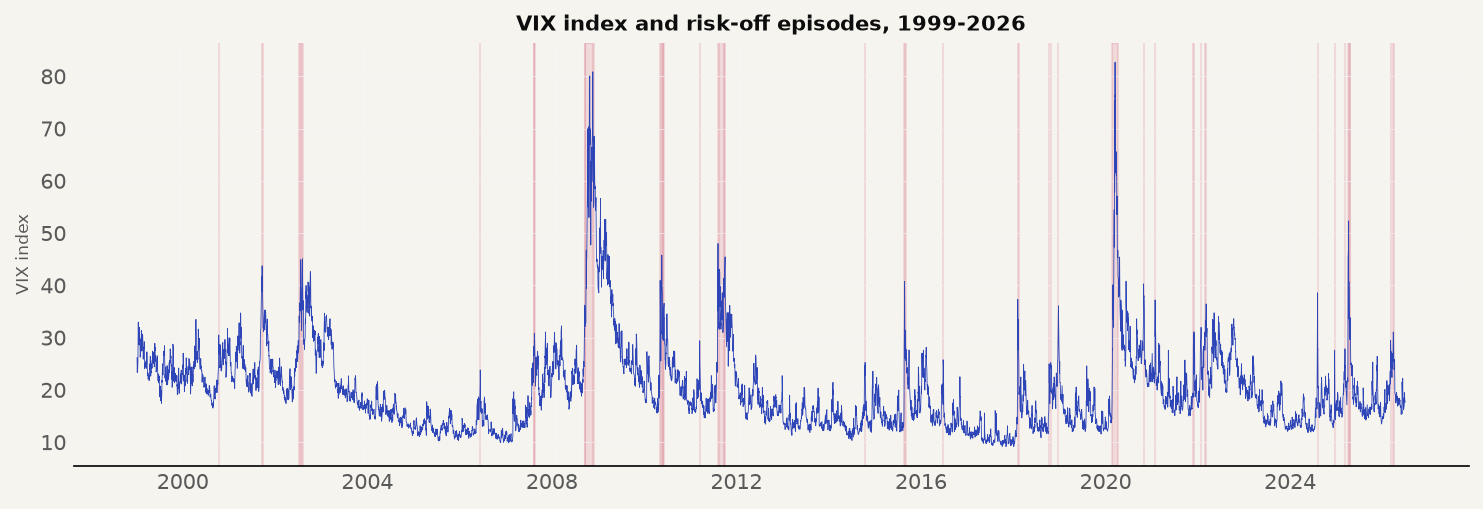
\includegraphics[width=\textwidth]{data/processed/var_results/figures/stylized_vix_risk_off.png}
  \caption{VIX and Risk-off Episodes, 1999--2026 (paper's Figure 1)}
  \label{fig:vix}
\end{figure}

\begin{figure}[H]
  \centering
  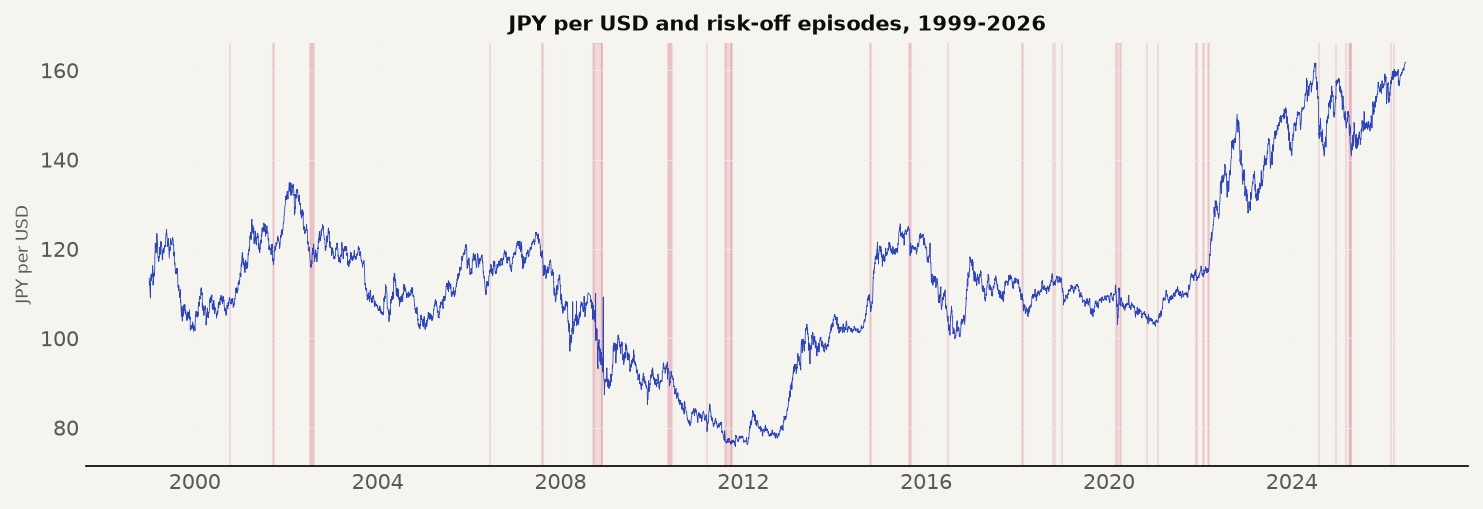
\includegraphics[width=\textwidth]{data/processed/var_results/figures/stylized_usdjpy_risk_off.png}
  \caption{USD/JPY Exchange Rate and Risk-off Episodes, 1999--2026 (paper's Figure 2)}
  \label{fig:usdjpy}
\end{figure}

\begin{figure}[H]
  \centering
  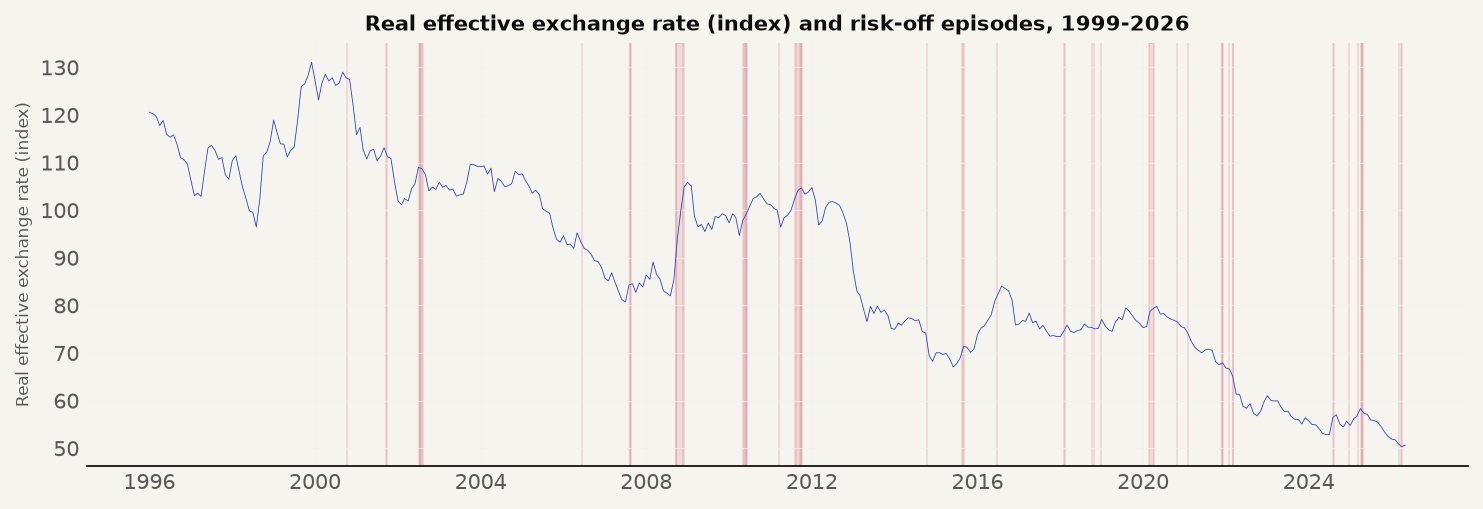
\includegraphics[width=\textwidth]{data/processed/var_results/figures/stylized_reer_risk_off.png}
  \caption{Japan's Real Effective Exchange Rate and Risk-off Episodes, 1999--2026 (paper's Figure 3)}
  \label{fig:reer}
\end{figure}

\subsubsection{Sovereign Yield and Spread}

The second group covers the bond market channels and contrasts directly with the paper's stylized facts. The paper shows JGB yields falling during risk-off episodes on purchases by domestic and foreign investors, and notes that the 10-year yield rose by at most 24 basis points during the COVID-19 episode from 24 February to 7 April 2020, evidence of how contained the flight-to-safety move was in Japanese debt \parencite{beirne_sugandi_2023}. Figure~\ref{fig:jgb} confirms the compression through 2020, yields falling from roughly 2 percent in 1999 to near zero by 2010 and below zero during the pandemic, and then shows the regime the paper could not observe, yields rising above 2.5 percent after 2023 as the Bank of Japan normalized policy. Figure~\ref{fig:us10y} extends the comparison the paper draws to the United States, Treasury yields declining in each episode through 2020, from above 6 percent in 2000 to near zero in 2020, then rising above 4 percent after 2021. The spread in Figure~\ref{fig:spread} widens through 2020, consistent with the paper's Appendix 1 panel, and after 2021 it narrows not because risk-off dynamics have changed but because both yields rise simultaneously under fundamentally different monetary policy regimes, the rate-differential dominance that the surveillance evidence attributes to the period \parencite{imf_2025}.

\begin{figure}[H]
  \centering
  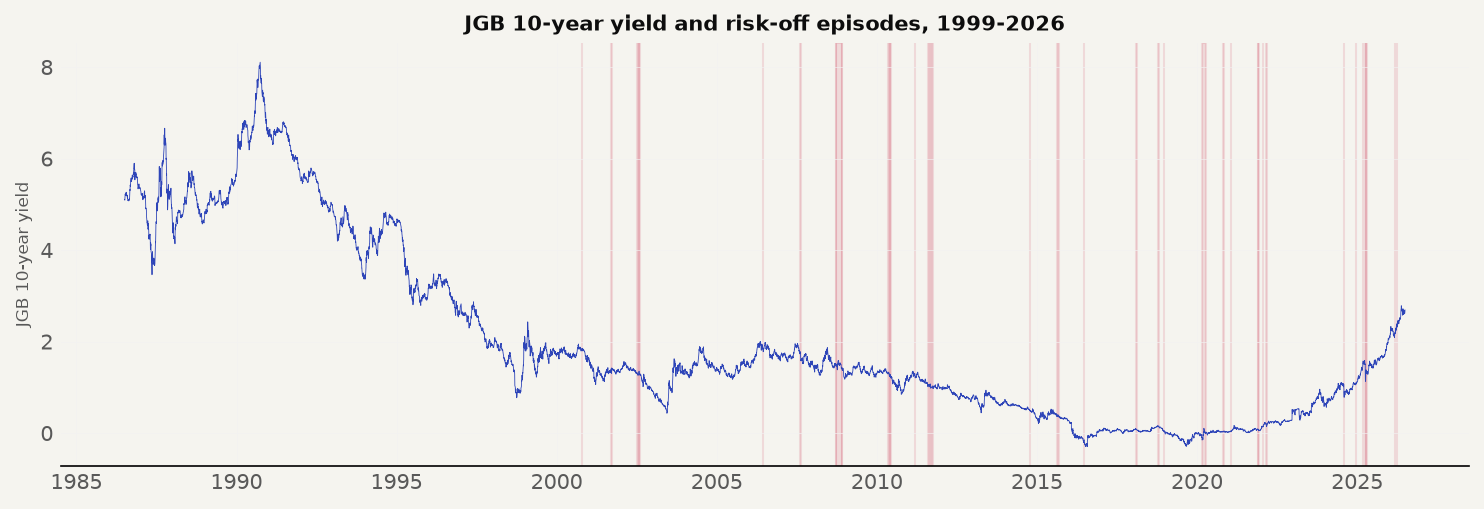
\includegraphics[width=\textwidth]{data/processed/var_results/figures/stylized_jgb10y_risk_off.png}
  \caption{10-Year JGB Yield and Risk-off Episodes, 1999--2026 (paper's Figure A1.1)}
  \label{fig:jgb}
\end{figure}

\begin{figure}[H]
  \centering
  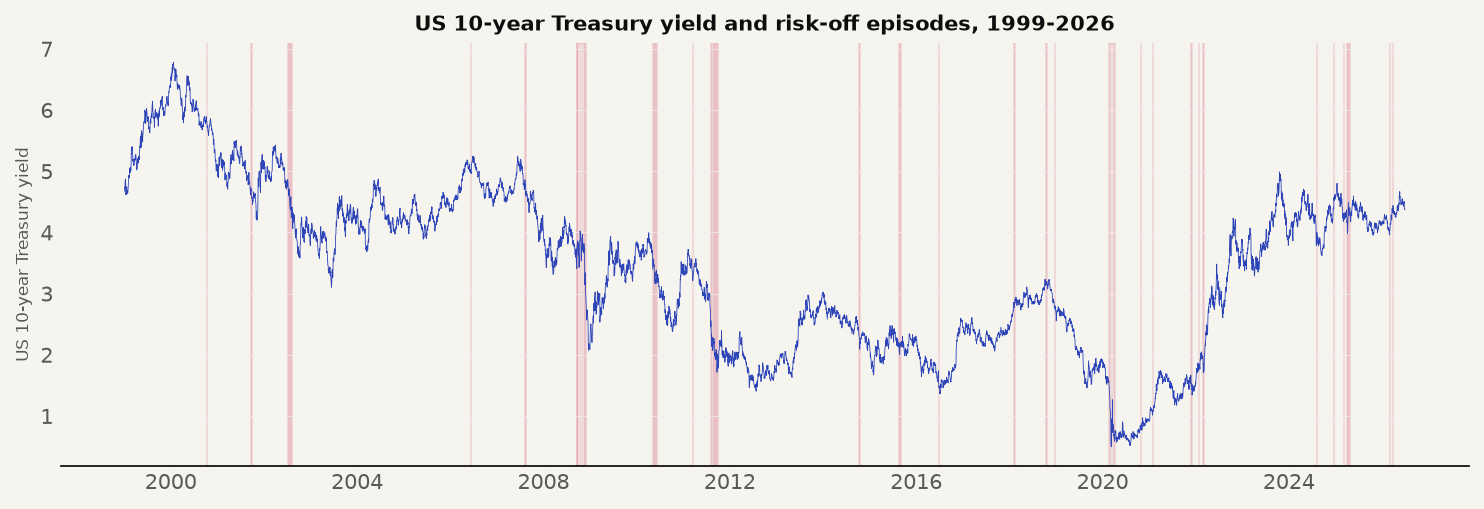
\includegraphics[width=\textwidth]{data/processed/var_results/figures/stylized_us10y_risk_off.png}
  \caption{US 10-Year Treasury Yield and Risk-off Episodes, 1999--2026}
  \label{fig:us10y}
\end{figure}

\begin{figure}[H]
  \centering
  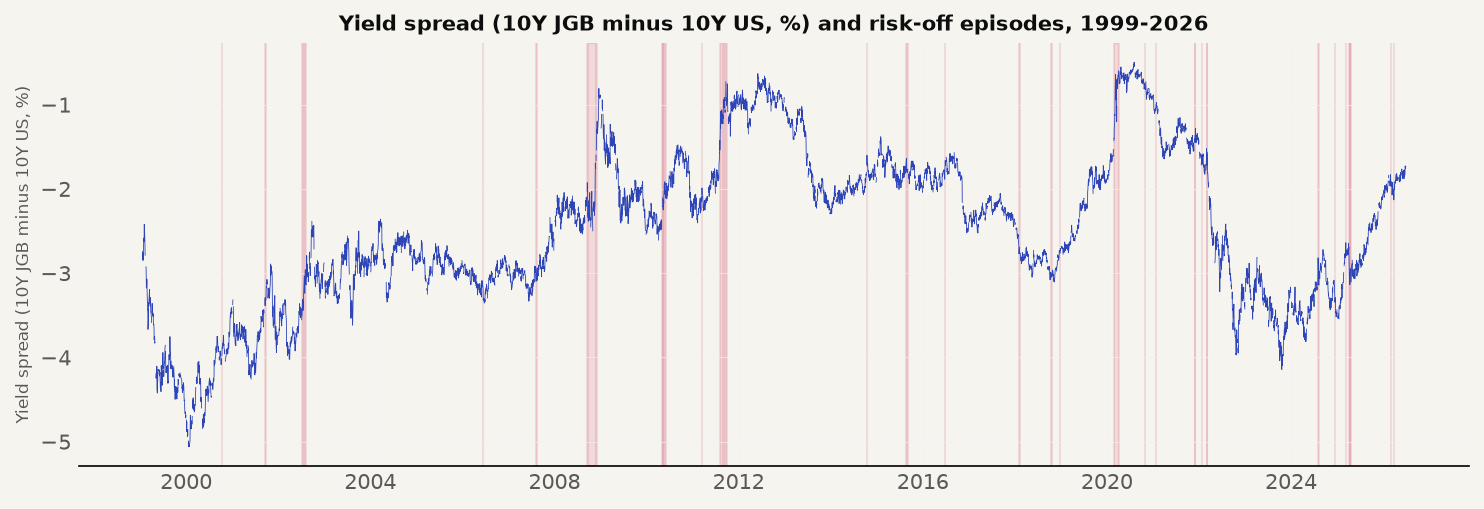
\includegraphics[width=\textwidth]{data/processed/var_results/figures/stylized_spread_risk_off.png}
  \caption{Yield Spread, 10-Year JGB Minus 10-Year US Treasury, and Risk-off Episodes, 1999--2026 (paper's Figure A1.7)}
  \label{fig:spread}
\end{figure}

\subsubsection{Equity Market}

The equity panel tests the paper's claim that Japanese equities are not safe haven assets, with the Nikkei falling during risk-off episodes in line with United States indices \parencite{beirne_sugandi_2023}. Figure~\ref{fig:nikkei} confirms the claim over the shared window, the index oscillating between 7,000 and roughly 30,000 for two decades and collapsing in the dot-com episode, the global financial crisis, the Tohoku shock, and the pandemic, and then shows the break, the index surging beyond 70,000 after 2023. A market that spent more than three decades regaining its 1989 peak doubled in the three years after 2023, a structural shift driven by corporate governance reforms, the Tokyo Stock Exchange's restructuring push, and the return of inflation to Japan after three decades of deflation. The equity market therefore behaves as the paper describes during risk-off episodes in both samples, and the level shift of the post-2023 surge enters the log index that the extended-period VAR uses, which is part of why the extended stock response should be read with the regime change in mind.

\begin{figure}[H]
  \centering
  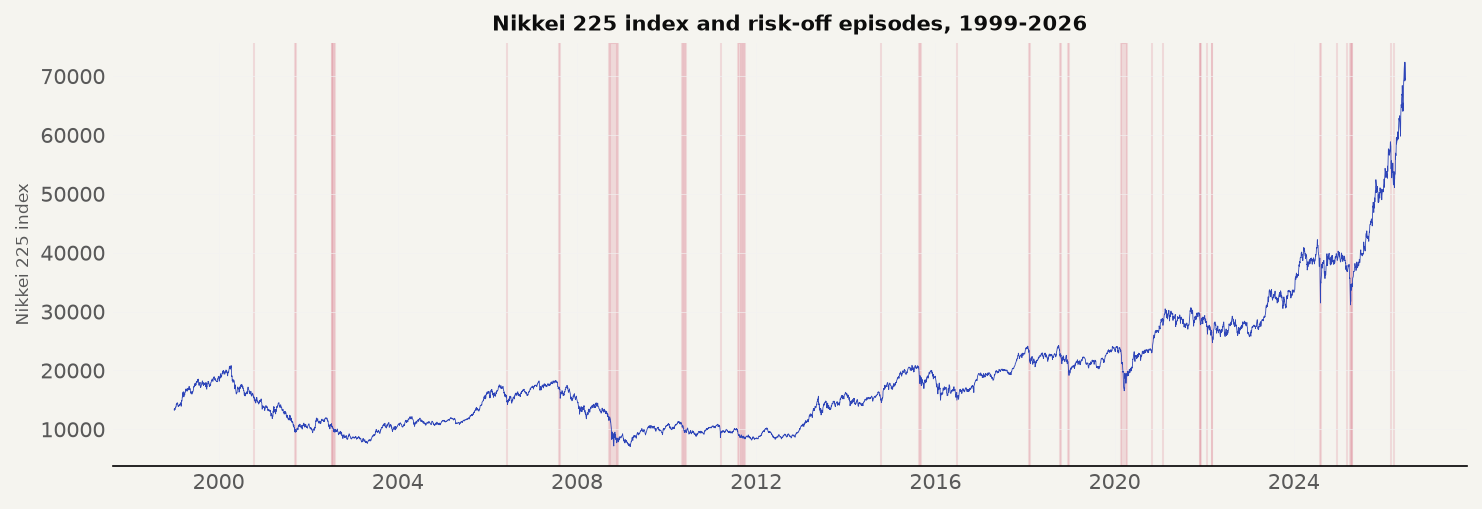
\includegraphics[width=\textwidth]{data/processed/var_results/figures/stylized_nikkei225_risk_off.png}
  \caption{Nikkei 225 Index and Risk-off Episodes, 1999--2026 (paper's Figure A1.2)}
  \label{fig:nikkei}
\end{figure}

\subsubsection{Capital Flows}

The capital flow panels contrast with the paper's stylized-facts expectations. The paper describes foreign investors reducing Japanese equity holdings during risk-off periods, other investment flows tending positive or increasing on repatriation, and Japanese investors bringing overseas funds back to domestic banking accounts \parencite{beirne_sugandi_2023}. The four capital flow series in Figures~\ref{fig:debtsec}, \ref{fig:equity}, \ref{fig:other}, and \ref{fig:direct} show no such systematic response, in either the shared window or the extension, the series are noisy and the risk-off bands do not line up with any consistent direction, with the other investment category spiking to nearly 29 percent of GDP in early 2020. The paper's own appendix panels A1.3 to A1.6 display the same visual story, so the raw data of both studies agree on the central point, the price channels respond to risk-off episodes and the volume channels do not, and the VAR results below confirm that the flow responses are statistically indistinguishable from zero.

\begin{figure}[H]
  \centering
  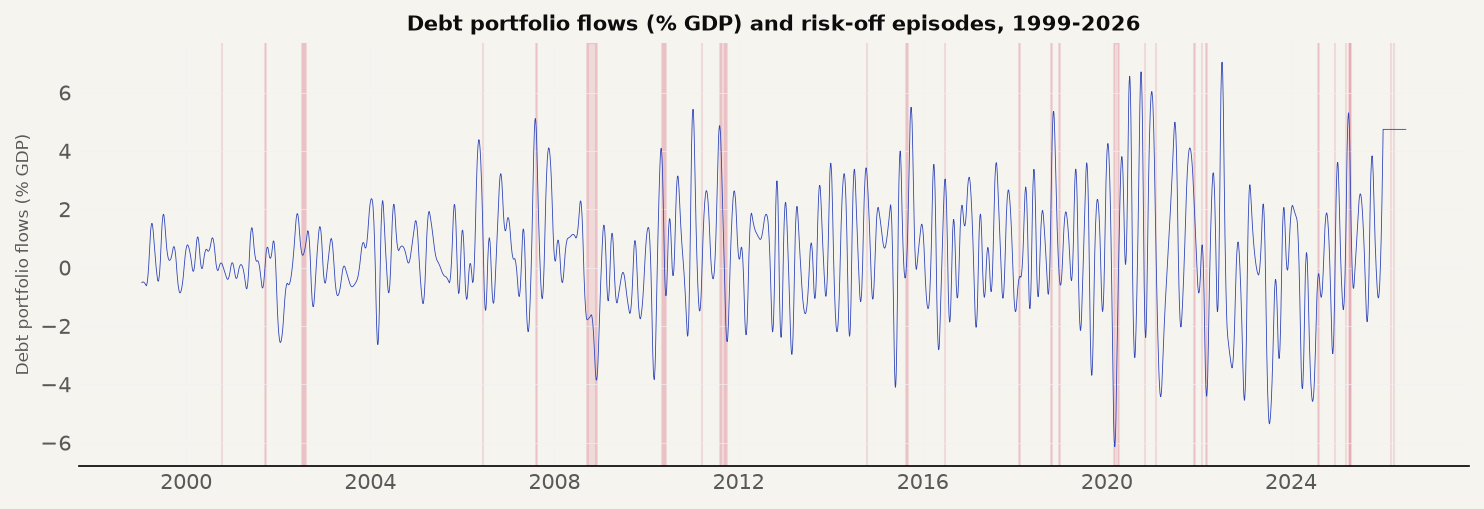
\includegraphics[width=\textwidth]{data/processed/var_results/figures/stylized_debtsecpct_risk_off.png}
  \caption{Portfolio Debt Flows and Risk-off Episodes, 1999--2026 (paper's Figure A1.3)}
  \label{fig:debtsec}
\end{figure}

\begin{figure}[H]
  \centering
  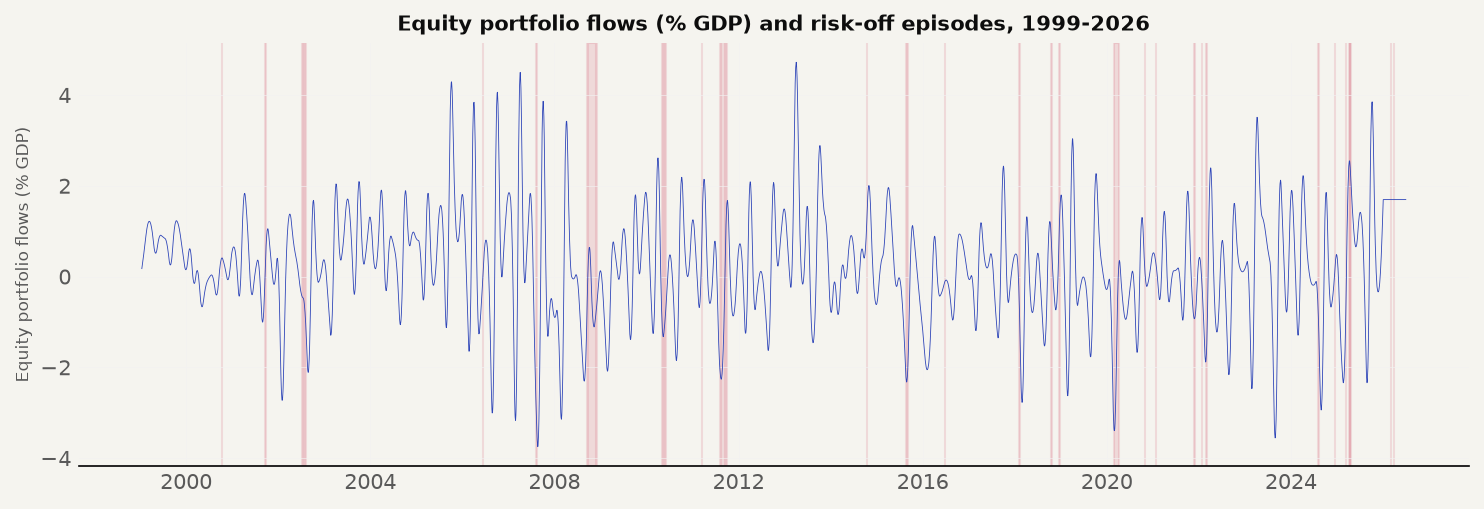
\includegraphics[width=\textwidth]{data/processed/var_results/figures/stylized_equitypct_risk_off.png}
  \caption{Portfolio Equity Flows and Risk-off Episodes, 1999--2026 (paper's Figure A1.4)}
  \label{fig:equity}
\end{figure}

\begin{figure}[H]
  \centering
  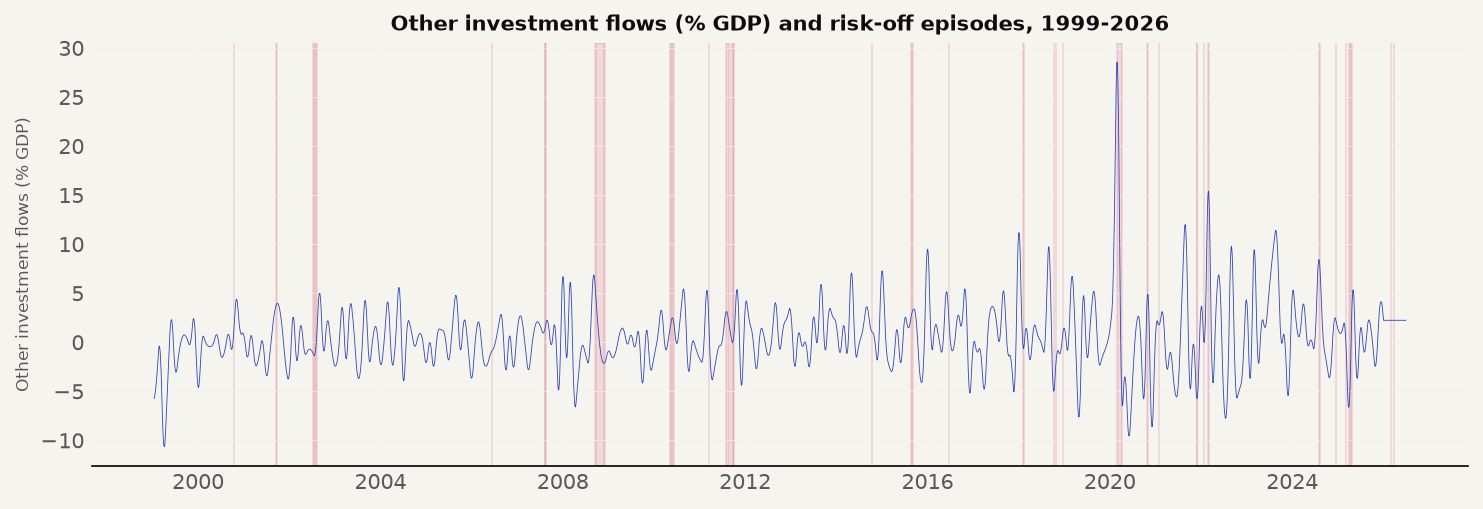
\includegraphics[width=\textwidth]{data/processed/var_results/figures/stylized_otherpct_risk_off.png}
  \caption{Other Investment Flows and Risk-off Episodes, 1999--2026 (paper's Figure A1.5)}
  \label{fig:other}
\end{figure}

\begin{figure}[H]
  \centering
  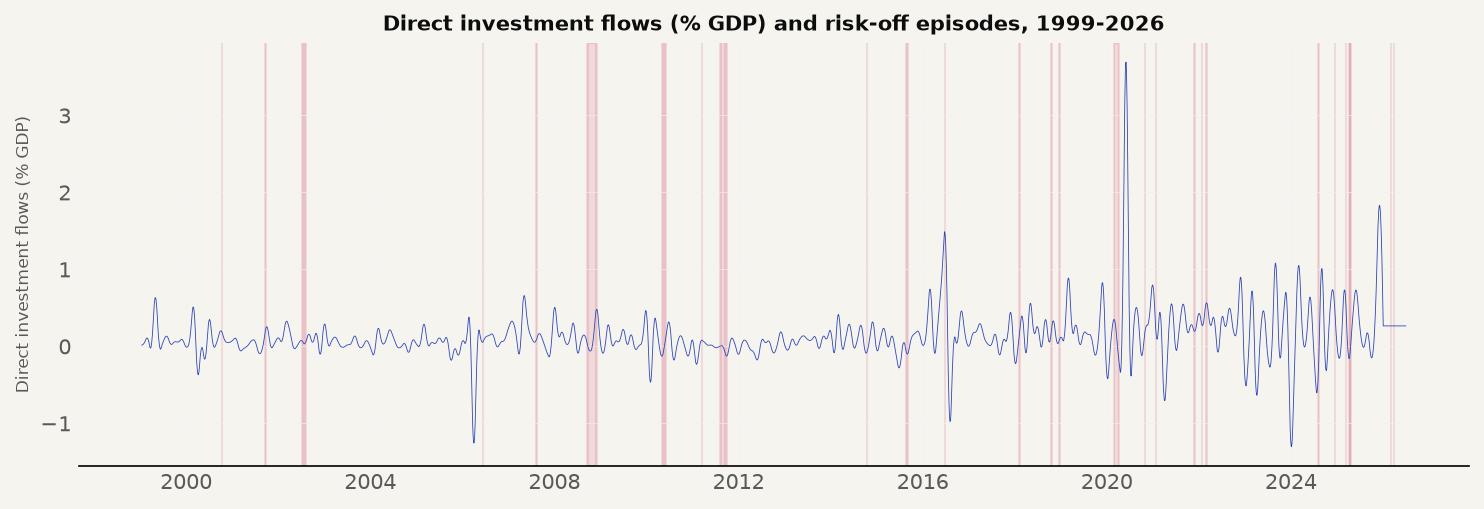
\includegraphics[width=\textwidth]{data/processed/var_results/figures/stylized_directpct_risk_off.png}
  \caption{Direct Investment Flows and Risk-off Episodes, 1999--2026 (paper's Figure A1.6)}
  \label{fig:direct}
\end{figure}

\subsubsection{Risk-off Episodes}

Table~\ref{tab:episodes} lists the risk-off episodes identified by the VIX rule over the full sample, and it contrasts with the paper's Table 1 in a precise way. The rule reproduces all fifteen of the paper's in-sample initial dates exactly, the 2000 dot-com crash, the 2001 attacks, the 2002 corporate scandals, the 2006 tensions, the 2007 BNP Paribas freeze, the 2008 Lehman failure, the 2010 flash crash, the 2011 Tohoku shock and debt ceiling crisis, the 2014 sell-off, the 2015 China crash, the 2016 Brexit vote, the 2018 volatility spike and trade war, and the 2020 COVID outbreak. The extension then adds the episodes the paper could not have observed, the Omicron episode of November 2021, the Russia-Ukraine episode of March 2022, the yen carry trade unwind of August 2024, the Federal Reserve hawkish pause of December 2024, the tariff episodes of March to April 2025, and the Middle East escalation of March 2026. The August 2024 episode is short but the most consequential of the extension, matching the carry trade unwind documented by \textcite{aquilina_lombardi_schrimpf_sushko_2024}.

\begin{table}[H]
  \centering
  \caption{Risk-off Episodes Identified by the VIX Rule, 1999--2026}
  \label{tab:episodes}
  \small
  \begin{tabular}{@{}l r p{8.2cm}@{}}
    \toprule
    Dates & Days & Event / Interpretation \\
    \midrule
Dates & Days & Event / Interpretation \\
Oct 12, 2000 & 1 & Dot-com crash / Tech sell-off \\
Sep 17, 2001 -- Sep 26, 2001 & 8 & 9/11 attacks \& aftermath \\
Jul 10, 2002 -- Aug 07, 2002 & 15 & Corporate scandals (WorldCom, Enron) \\
Jun 13, 2006 & 1 & Geopolitical tensions (Iran / NK) \\
Aug 09, 2007 -- Aug 17, 2007 & 6 & BNP Paribas freezes funds / GFC onset \\
Sep 17, 2008 -- Dec 01, 2008 & 46 & Global Financial Crisis (Lehman collapse) \\
May 06, 2010 -- Jun 07, 2010 & 14 & Flash Crash / Eurozone debt crisis \\
Mar 16, 2011 & 1 & Tohoku earthquake \& tsunami \\
Aug 04, 2011 -- Aug 26, 2011 & 16 & US debt ceiling / Eurozone sovereign crisis \\
Sep 06, 2011 -- Oct 03, 2011 & 8 & US debt ceiling / Eurozone sovereign crisis \\
Oct 13, 2014 -- Oct 16, 2014 & 3 & Ebola / Oil price collapse \\
Aug 21, 2015 -- Sep 04, 2015 & 9 & China crash (Black Monday) / Brexit \\
Jun 24, 2016 & 1 & China crash (Black Monday) / Brexit \\
Feb 05, 2018 -- Feb 13, 2018 & 7 & Volmageddon (Volatility spike) \\
Oct 11, 2018 & 1 & Trade war / Tech sell-off \\
Oct 24, 2018 & 1 & Trade war / Tech sell-off \\
Dec 21, 2018 -- Dec 24, 2018 & 2 & Trade war / Tech sell-off \\
Feb 24, 2020 -- Apr 07, 2020 & 32 & COVID-19 global pandemic \\
Oct 28, 2020 -- Oct 30, 2020 & 3 & COVID-19 pandemic \\
Jan 27, 2021 & 1 & GameStop short squeeze / Retail mania \\
Nov 26, 2021 -- Dec 03, 2021 & 3 & Omicron variant / Fed hawkish pivot \\
Jan 25, 2022 -- Jan 26, 2022 & 2 & Omicron variant / Fed hawkish pivot \\
Mar 01, 2022 -- Mar 08, 2022 & 3 & Russia-Ukraine war / Commodity crisis \\
Aug 05, 2024 -- Aug 07, 2024 & 3 & Yen carry trade unwind / Global sell-off \\
Dec 18, 2024 & 1 & Fed hawkish pause / BOJ policy divergence \\
Mar 10, 2025 & 1 & "America First" trade policy / Tariff war \\
Apr 03, 2025 -- Apr 21, 2025 & 9 & "America First" trade policy / Tariff war \\
Mar 06, 2026 & 1 & Iran conflict / Middle East escalation \\
Mar 27, 2026 -- Mar 30, 2026 & 2 & Iran conflict / Middle East escalation \\
    \bottomrule
  \end{tabular}
  \caption*{\textit{Note.} A risk-off event is a day on which the VIX exceeds its 60-day moving average by at least 10 points. Episodes merge events separated by no more than ten days.}
\end{table}

\subsection{Stationarity and Lag Selection}

The descriptive record is complemented by the formal diagnostics that support the specification. Table~\ref{tab:adf} reports augmented Dickey-Fuller tests for both samples. The risk-off indicator, the uncertainty index, and the four capital flow variables reject a unit root at the 5 percent level in both periods. The spread, real GDP, the REER, and the stock index do not, which is the expected pattern for slowly moving levels series in a system estimated with a linear time trend. The model is estimated in levels, which is standard in the macro VAR literature \parencite{sims_1980,lutkepohl_2005}, and the trend-stationary reading of the levels variables is supported by the trend term in the exogenous matrix.

\begin{table}[htbp]
  \centering
  \caption{Augmented Dickey-Fuller Tests at the 5 Percent Level}
  \label{tab:adf}
  \small
  \begin{tabular}{@{}l l r r r l@{}}
    \toprule
    Variable & Period & ADF Statistic & p-value & 5\% Critical Value & Stationary \\
    \midrule
Risk-off & 1999-2021 & -10.4830 & 0.0000 & -2.8621 & Yes \\
Log (WUI) & 1999-2021 & -7.2948 & 0.0000 & -2.8621 & Yes \\
Spread & 1999-2021 & -2.0508 & 0.2648 & -2.8621 & No \\
Log (RGDP) & 1999-2021 & -1.8444 & 0.3586 & -2.8621 & No \\
Log (REER) & 1999-2021 & -1.0876 & 0.7200 & -2.8621 & No \\
Log (Nikkei) & 1999-2021 & -0.8748 & 0.7962 & -2.8621 & No \\
Debtsec & 1999-2021 & -10.4345 & 0.0000 & -2.8621 & Yes \\
Equity & 1999-2021 & -9.3888 & 0.0000 & -2.8621 & Yes \\
Other & 1999-2021 & -10.0058 & 0.0000 & -2.8621 & Yes \\
Direct & 1999-2021 & -8.9080 & 0.0000 & -2.8621 & Yes \\
Risk-off & 1999-2026 & -12.8264 & 0.0000 & -2.8620 & Yes \\
Log (WUI) & 1999-2026 & -6.4418 & 0.0000 & -2.8620 & Yes \\
Spread & 1999-2026 & -2.3413 & 0.1590 & -2.8620 & No \\
Log (RGDP) & 1999-2026 & -1.7015 & 0.4303 & -2.8620 & No \\
Log (REER) & 1999-2026 & -0.1465 & 0.9446 & -2.8620 & No \\
Log (Nikkei) & 1999-2026 & 0.6358 & 0.9885 & -2.8620 & No \\
Debtsec & 1999-2026 & -9.7198 & 0.0000 & -2.8620 & Yes \\
Equity & 1999-2026 & -10.2960 & 0.0000 & -2.8620 & Yes \\
Other & 1999-2026 & -10.7074 & 0.0000 & -2.8620 & Yes \\
Direct & 1999-2026 & -10.2089 & 0.0000 & -2.8620 & Yes \\
    \bottomrule
  \end{tabular}
\end{table}

The lag selection procedure is documented in Section 3 as a process of elimination, and the diagnostics are reported in Figure~\ref{fig:adf}, Figure~\ref{fig:lag}, and Table~\ref{tab:lag}. The daily AIC declines through the search boundary of 20 in both samples, with small local increases at the upper lags, and selects the boundary lag regardless of the cap. The monthly BIC selects two lags for the paper period and three lags for the extended sample, and the selected specifications reproduce the sign, shape, and peak timing of the paper's monthly figures.

\begin{figure}[htbp]
  \centering
  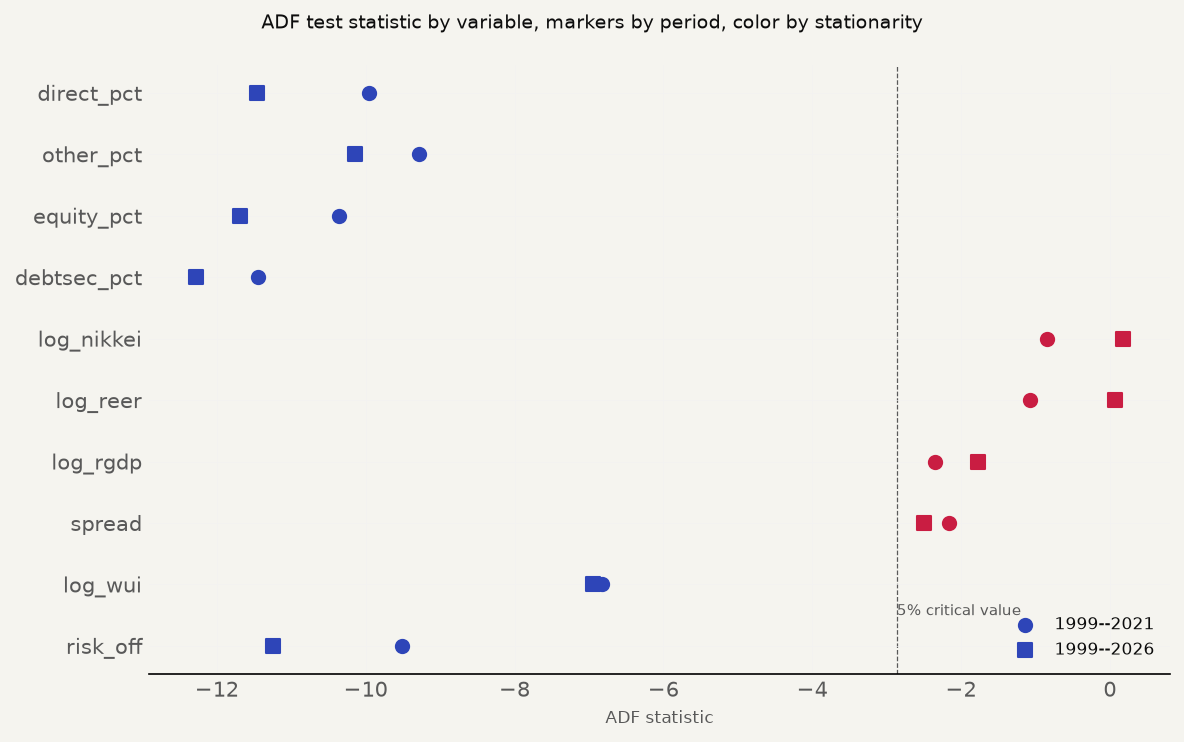
\includegraphics[width=\textwidth]{data/processed/var_results/figures/infographics_adf_stationarity.png}
  \caption{Stationarity Diagnostics}
  \label{fig:adf}
  \caption*{\textit{Note.} Circle and square markers distinguish the two sample periods. Blue indicates rejection of the unit root at the 5 percent level, red indicates failure to reject.}
\end{figure}

\begin{figure}[htbp]
  \centering
  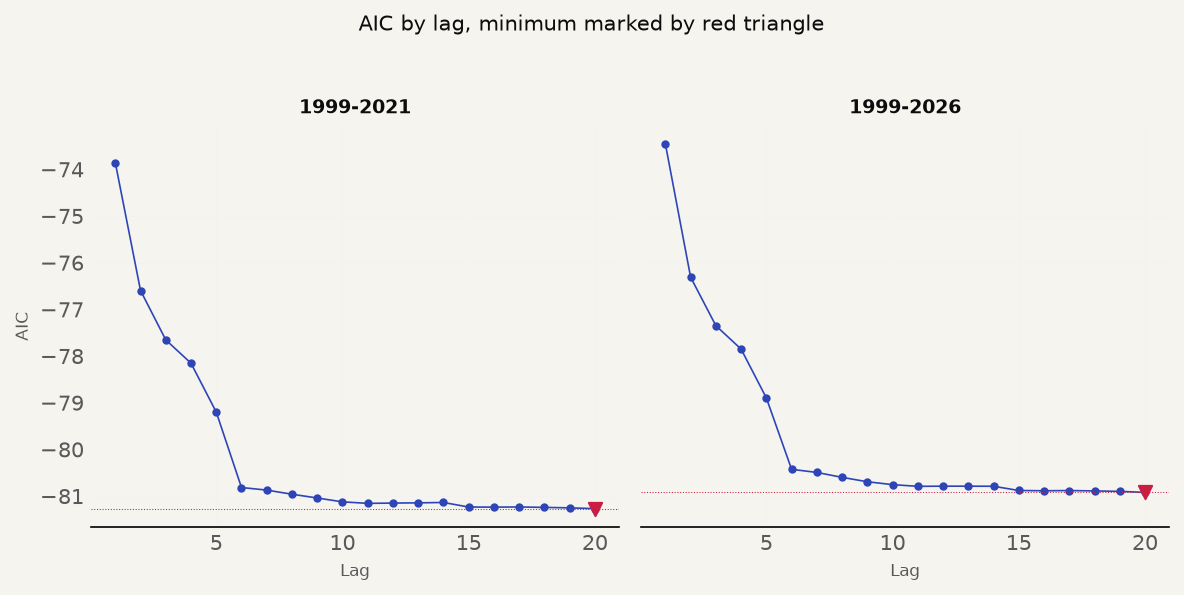
\includegraphics[width=\textwidth]{data/processed/var_results/figures/infographics_lag_selection.png}
  \caption{Lag Selection Diagnostics}
  \label{fig:lag}
\end{figure}

\begin{table}[htbp]
  \centering
  \caption{Daily AIC by Lag for Both Samples}
  \label{tab:lag}
  \small
  \begin{tabular}{@{}r r r@{}}
    \toprule
    Lag & AIC 1999--2021 & AIC 1999--2026 \\
    \midrule
1 & -73.8544 & -73.4575 \\
2 & -76.5963 & -76.3110 \\
3 & -77.6532 & -77.3494 \\
4 & -78.1539 & -77.8516 \\
5 & -79.2003 & -78.8975 \\
6 & -80.8161 & -80.4265 \\
7 & -80.8712 & -80.4928 \\
8 & -80.9599 & -80.5986 \\
9 & -81.0404 & -80.6922 \\
10 & -81.1231 & -80.7544 \\
11 & -81.1555 & -80.7904 \\
12 & -81.1491 & -80.7875 \\
13 & -81.1447 & -80.7874 \\
14 & -81.1364 & -80.7892 \\
15 & -81.2342 & -80.8798 \\
16 & -81.2359 & -80.8860 \\
17 & -81.2328 & -80.8810 \\
18 & -81.2415 & -80.8891 \\
19 & -81.2517 & -80.8988 \\
20 & -81.2686 & -80.9200 \\
    \bottomrule
  \end{tabular}
  \caption*{\textit{Note.} The AIC declines through the search boundary in both samples, with small local increases at the upper lags. The monthly tier uses the BIC, which selects two lags for the paper period and three for the extended sample.}
\end{table}

\subsection{Impulse Response Results, Paper Period}

The diagnostics above settle the specification, and the estimated responses follow. Figure~\ref{fig:irf_daily_paper} presents the daily restricted impulse responses for the paper period, and Figure~\ref{fig:irf_monthly_paper} the monthly restricted responses. Each panel shows the response of one endogenous variable to a one-standard-deviation risk-off shock, with the point estimate as a solid line and the 95 percent Monte Carlo band as shading. The per-variable results below compare each response with the paper's published figures.

\begin{figure}[htbp]
  \centering
  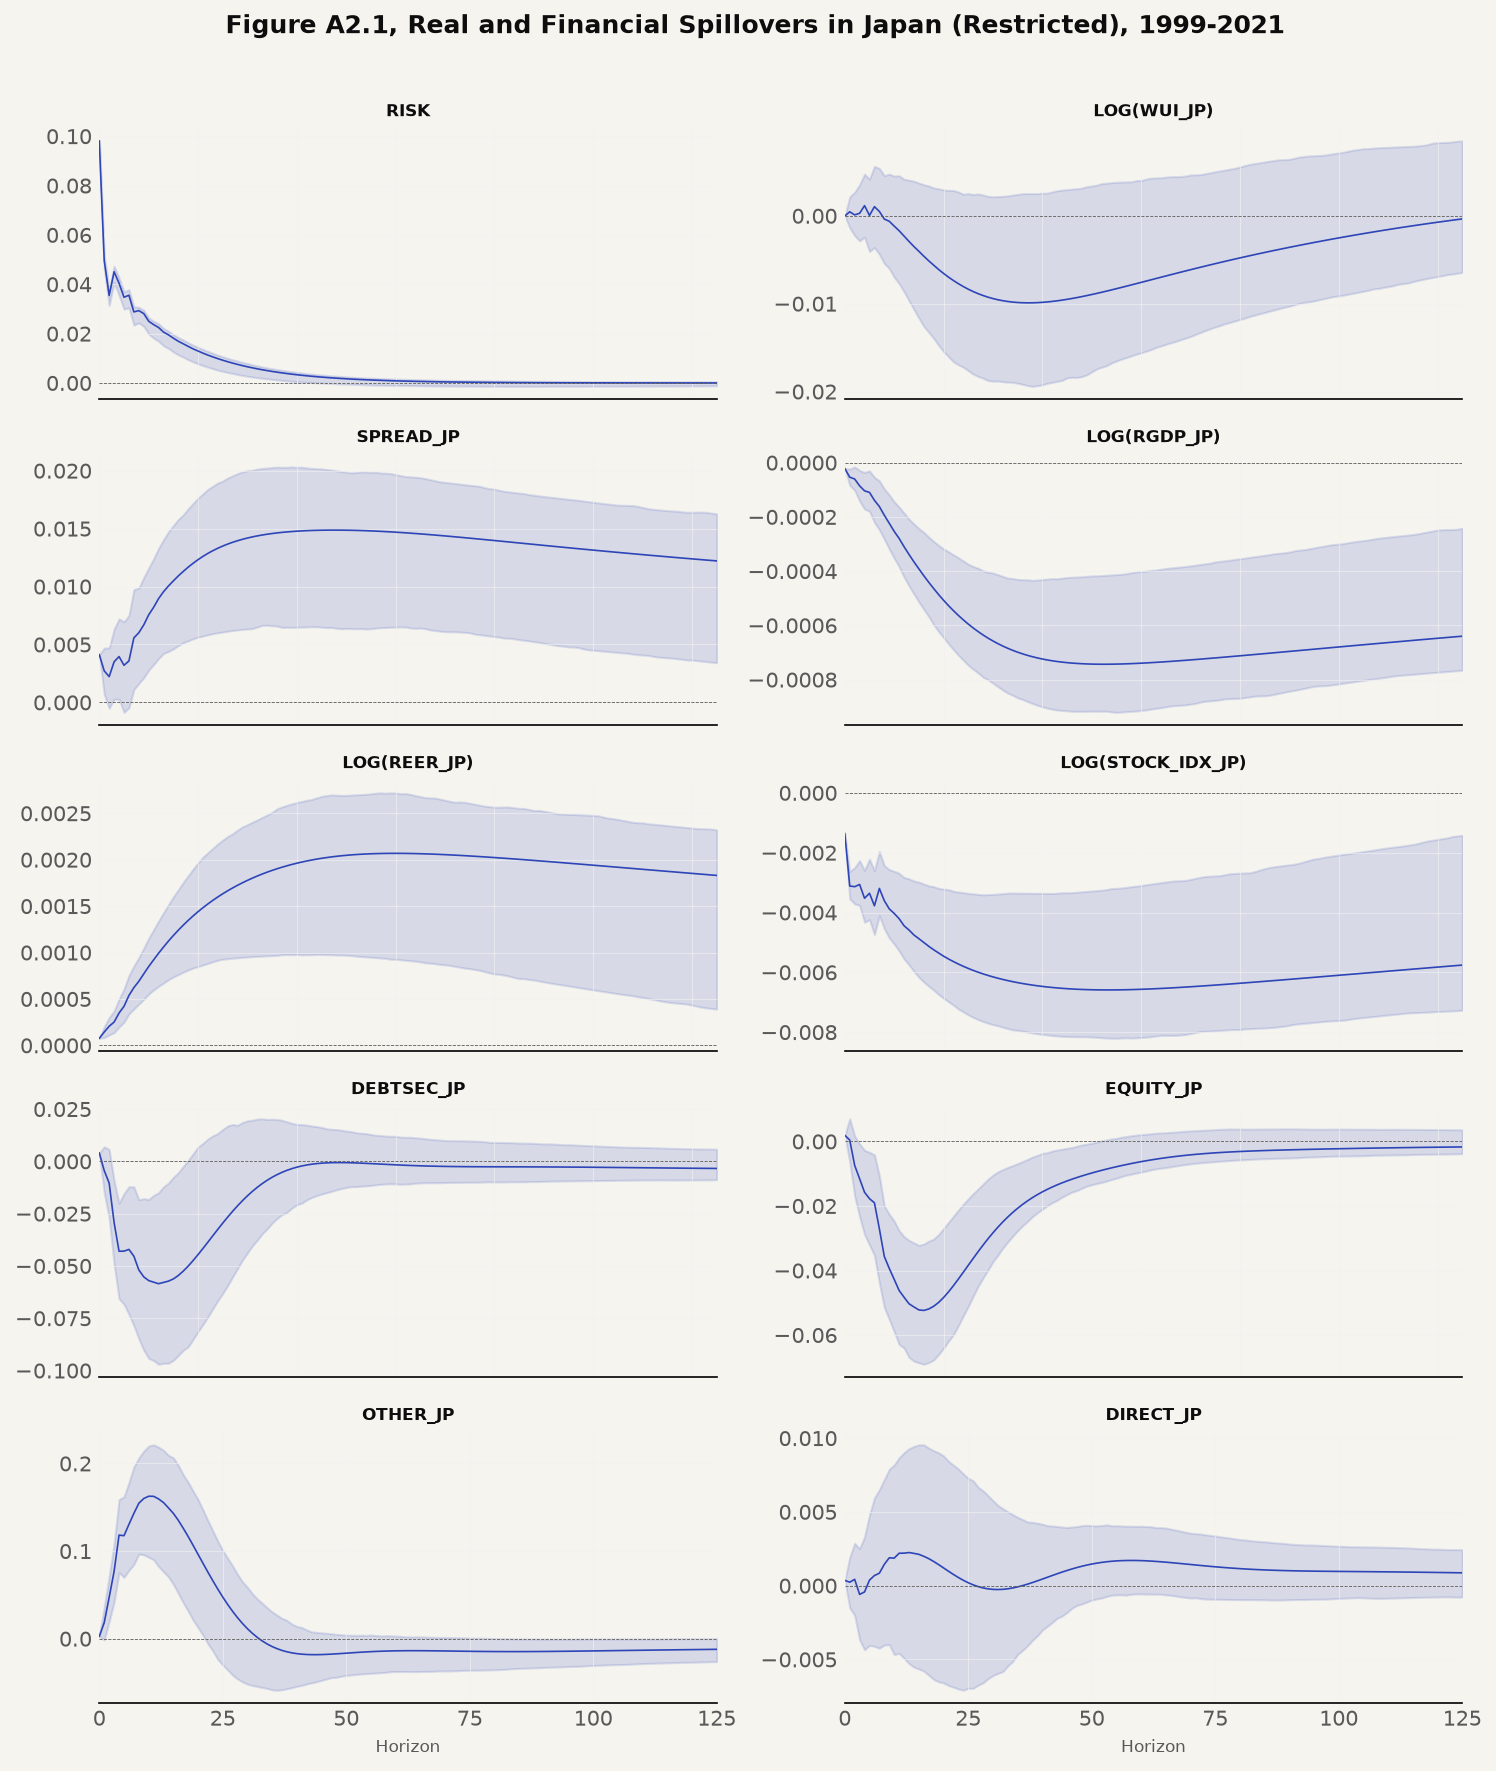
\includegraphics[width=\textwidth]{data/processed/var_results/figures/irf_grid_daily_restricted_paper.png}
  \caption{Daily Restricted Impulse Responses, Paper Period (paper's Figure A2.1)}
  \label{fig:irf_daily_paper}
\end{figure}

\begin{figure}[htbp]
  \centering
  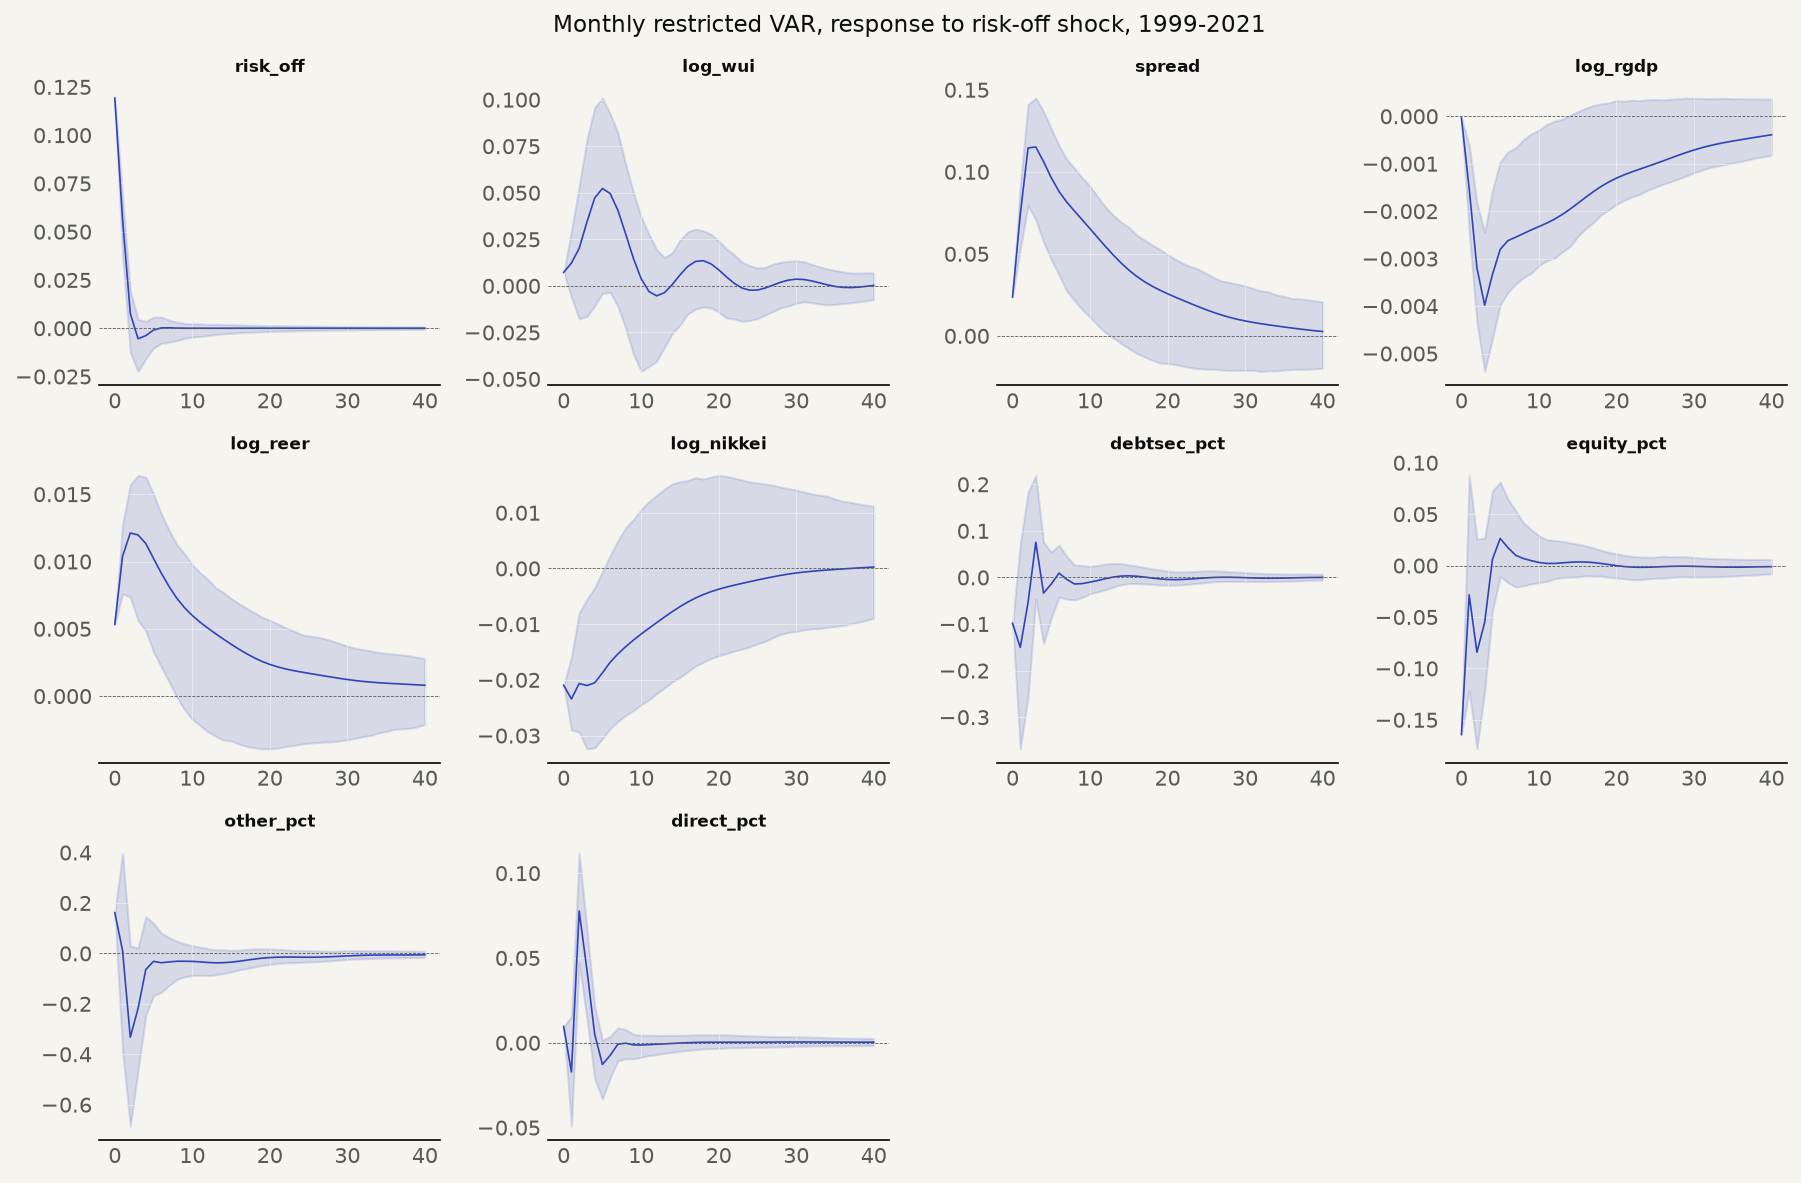
\includegraphics[width=\textwidth]{data/processed/var_results/figures/irf_grid_monthly_restricted_paper.png}
  \caption{Monthly Restricted Impulse Responses, Paper Period (paper's Appendix 4)}
  \label{fig:irf_monthly_paper}
\end{figure}

\subsubsection{Risk-off Indicator}

The risk-off self-response starts at 0.098, against the paper's 0.10, and decays toward zero over 125 trading days, with the bulk of the decay complete within 25 trading days. The two estimates agree on the dynamics of the exogenous impulse, which is the simplest equation in the system under the block exogeneity restriction. This is a match.

\subsubsection{World Uncertainty Index}

The paper's daily WUI response rises to a positive plateau of approximately 0.0017. The replication's daily response goes the other way, reaching a trough of approximately --0.010 around day 40 and returning to zero. The monthly specification is no kinder, with the replication peaking at 0.052 at month 5 against the paper's shallow dip to --0.003 at month 7. The WUI response disagrees with the paper at both frequencies, and this is the one clean failure of the replication. The sign of the WUI response depends on whether the episode is global or foreign-specific, because Japan reads as the safe haven during European debt crises and US rate scares, and the interpolation of the quarterly series amplifies the COVID spike-crash sequence into a steep daily decline. The paper's own daily and monthly WUI responses have opposite signs from each other, so the frequency dependence is present in their data as well.

\subsubsection{Sovereign Bond Spread}

The spread response is positive and persistent in both studies. The replication peaks at 0.015 around day 50 and decays to 0.012 by day 125, against the paper's peak of 0.010 decaying to 0.007. The monthly numbers carry the same story, with the replication starting at 0.024, spiking to 0.115 at month 3, and decaying to 0.003, against the paper's start of 0.04, spike of 0.075, and decay to 0.01. The magnitude runs about 1.5 times the paper's peak in both specifications, a consistent scaling difference driven by shock size rather than structural divergence. The directional pattern, the peak timing, and the persistence all match.

\subsubsection{Real GDP}

The daily restricted RGDP response is negative at every horizon, with the 95 percent band entirely below zero. At the first day the response is --0.000053, the trough of --0.000743 occurs around day 50 with a band from --0.000916 to --0.000418, and the response is --0.000640 at day 125. The paper troughs at --0.0006 around day 45 with confidence intervals below zero. The magnitudes are close enough to classify the daily comparison as a match, and the monthly restricted model reinforces it, reaching --0.003980 at month 3, remaining significant through month 6, marginal at month 12 with the upper band bound at --0.000104, and statistically indistinguishable from zero by month 24. The monthly trough is earlier and roughly twice as deep as the paper's, which carries the partial designation at the monthly frequency. This is the headline result of the replication, and it depends on the vintage data, since on current-vintage GDP the sign flips positive.

\subsubsection{Real Effective Exchange Rate}

The yen's safe-haven appreciation is the paper's central mechanism, and it reproduces cleanly. The replication's daily REER response reaches 0.002 at day 50 against the paper's 0.0008 plateau, and the monthly response peaks at 0.012 at month 3 against the paper's 0.005 at months 3 to 4. The direction is identical and the peak timing aligns in both frequencies. The REER channel is the most robust result in the replication, with every specification producing the expected appreciation.

\subsubsection{Stock Market Index}

The daily stock response diverges in one detail. The paper shows a small initial positive blip of 0.0005, the surge to safety, followed by a decline to --0.001. The replication is negative from the impact day, starting at --0.0014 and reaching --0.0066 at day 50. The monthly comparison restores the pattern, with the replication starting at --0.021 and recovering to 0.0002 by month 40 against the paper's start of --0.017 recovering to --0.004. The daily comparison is a partial match and the monthly is a match. The missing blip affects a movement that disappears within five trading days, and the economically meaningful negative trajectory replicates at both frequencies.

\subsubsection{Portfolio Debt Flows}

The debt flow response is a partial match at both frequencies. The daily estimate dips to --0.058 around day 12 and settles near zero, and the monthly estimate starts at --0.098 against the paper's 0.06, with both volatile and converging to zero. The long-run null replicates, which is the result that matters for the paper's conclusion, and it tells the same story as the theory, namely that the flight-to-safety mechanism operates through price channels rather than measurable portfolio volumes.

\subsubsection{Portfolio Equity Flows}

The daily equity comparison diverges in magnitude, with the replication troughing at --0.052 around day 16 against the paper's --0.006 at day 40, roughly nine times deeper at the trough with the same recovery direction. The monthly specification restores the pattern, with the replication showing an impact of --0.164, a trough of --0.055 at month 3, and a rebound to 0.026, against the paper's --0.065 at month 4 and 0.025 rebound. The daily is a partial match and the monthly is a match.

\subsubsection{Other Investment}

Other investment is the only clean mismatch among the capital flows. The paper dips and then peaks at 0.010 at day 50, while the replication spikes to 0.163 at day 10 and reaches --0.017 at day 50, a phase reversal between the paper's late peak and the replication's early spike. The variable is the catch-all category of the financial account, the highest-variance series in the model, and the phase difference is consistent with a source-data effect, since the Bank of Japan's BPM6 classification may group components differently than the paper's IMF IFS source.

\subsubsection{Direct Investment}

Direct investment is the exception among the capital flows. The daily trajectory aligns with the paper, reaching 0.0015 at day 50 and settling near 0.001 against the paper's dip to --0.002 and plateau at 0.001. The monthly specification finds the only statistically significant capital flow response in the entire analysis, with direct investment responding 0.043 at month 3 under the restricted specification and 0.036 under the unrestricted specification, both with bands excluding zero. Of the 40 flow-horizon entries in the significance table, exactly two reach the 95 percent threshold, and both are direct investment at the three-month horizon. The contrast with the paper's blanket null for capital flows is worth noting, since direct investment reflects long-horizon commitments that the theory would predict to be insulated from short-term risk-off dynamics.

\subsection{Robustness}

The paper-period results are checked against the unrestricted specification. Figure~\ref{fig:irf_daily_unrestricted_paper} presents the daily unrestricted grid, corresponding to the paper's Appendix 3. Removing the block exogeneity constraint widens the confidence bands but does not change the directional patterns of the restricted results. The unrestricted specification diverges from the restricted specification on current-vintage data, a divergence that is itself a finding about the sensitivity of the recursive identification to GDP data revisions.

\begin{figure}[htbp]
  \centering
  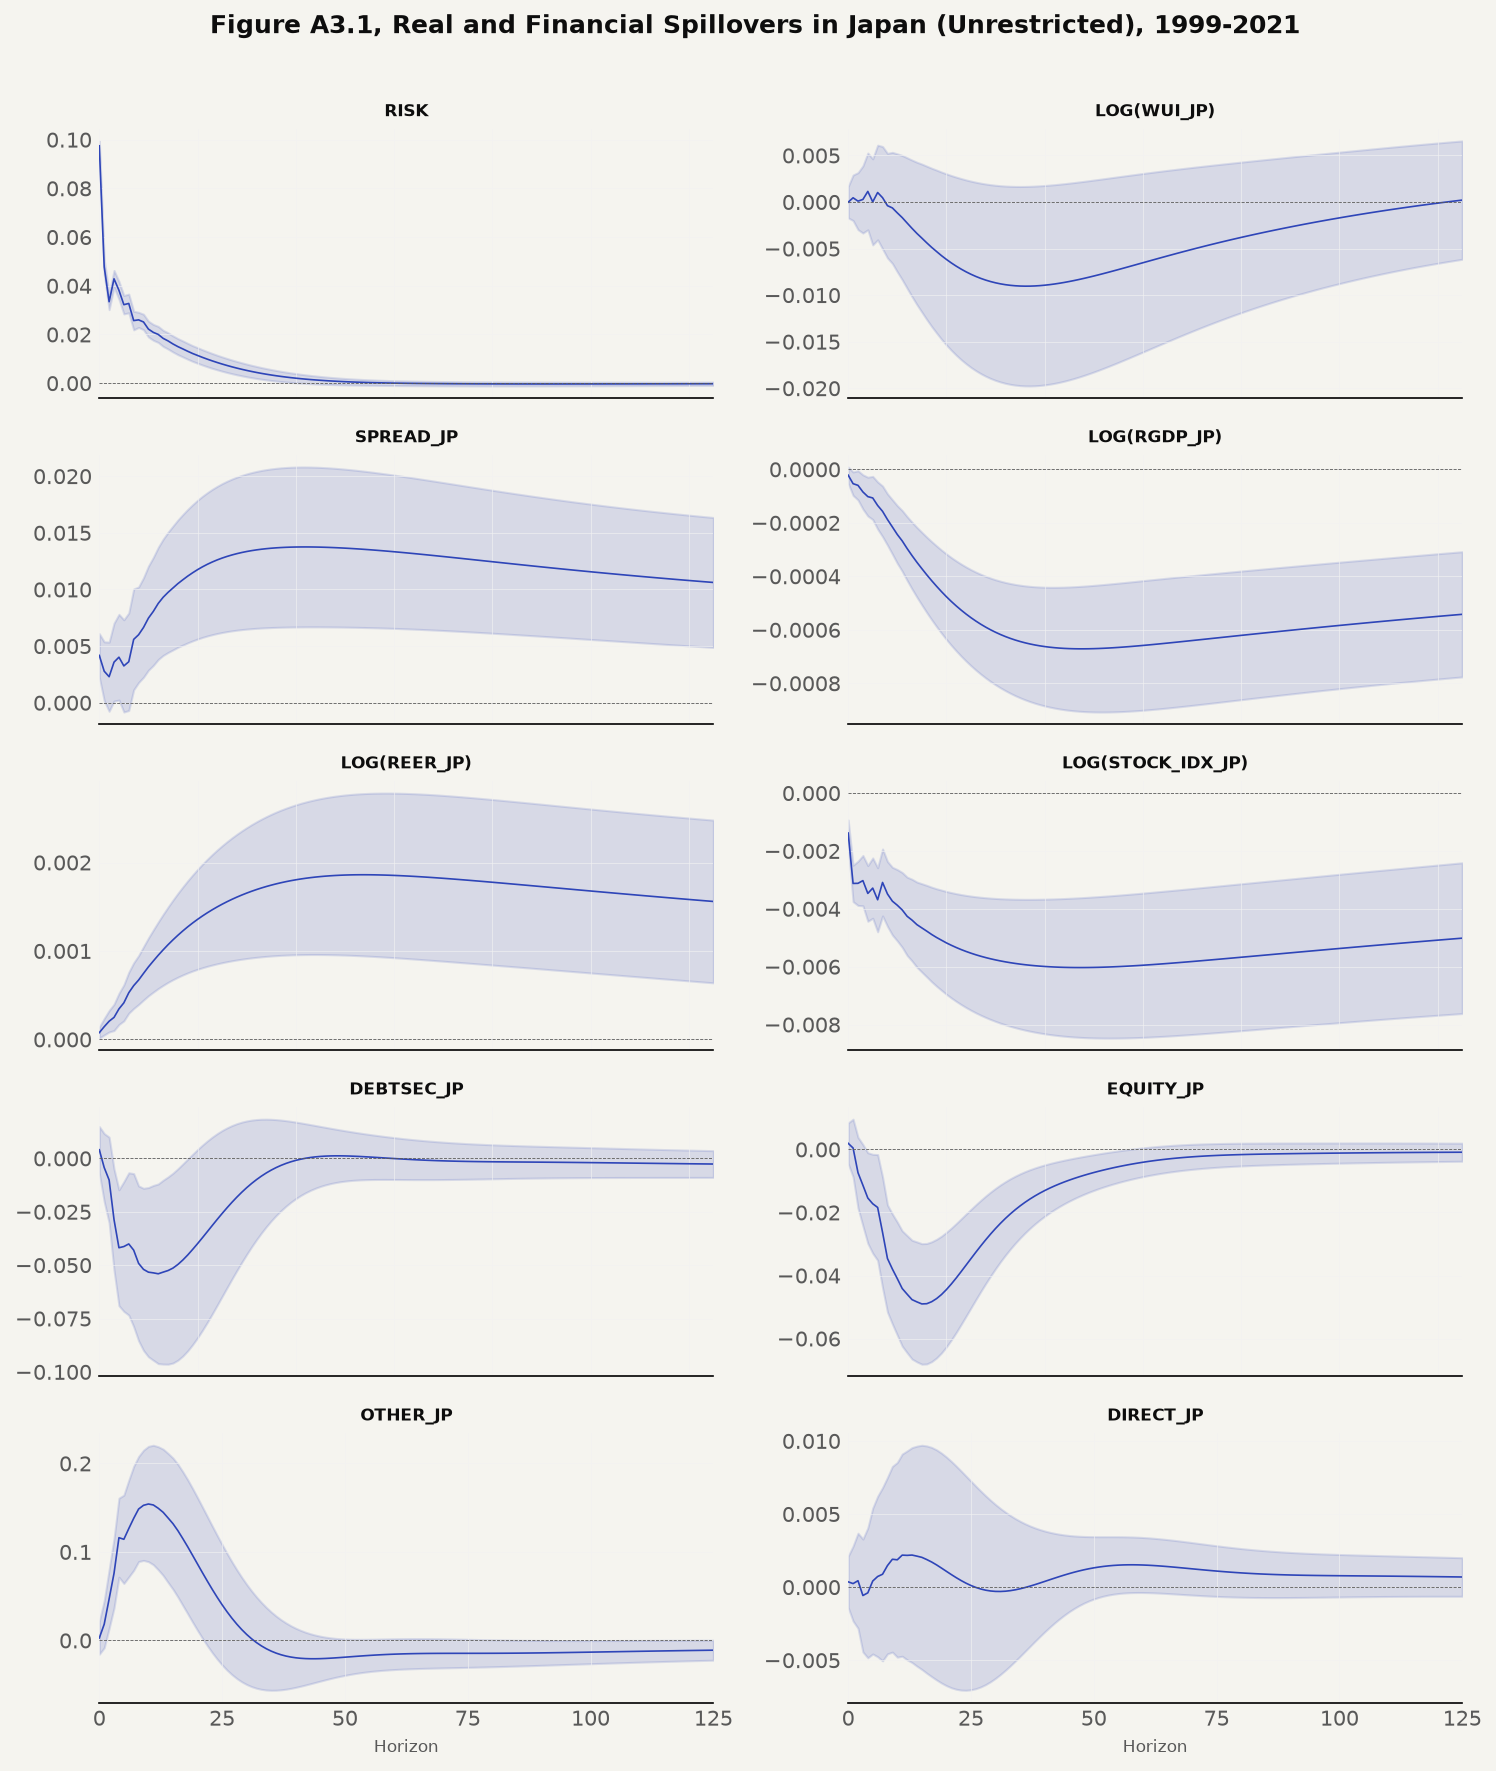
\includegraphics[width=\textwidth]{data/processed/var_results/figures/irf_grid_daily_unrestricted_paper.png}
  \caption{Daily Unrestricted Impulse Responses, Paper Period (paper's Figure A3.1)}
  \label{fig:irf_daily_unrestricted_paper}
\end{figure}

The monthly unrestricted specification was estimated as the corresponding robustness check at the lower frequency. Figure~\ref{fig:irf_monthly_unrestricted_paper} presents the grid. The monthly unrestricted responses match the restricted monthly responses closely, with the same widening of the confidence bands on the flow variables, and the same divergence from the restricted specification on current-vintage data documented for the daily tier.

\begin{figure}[htbp]
  \centering
  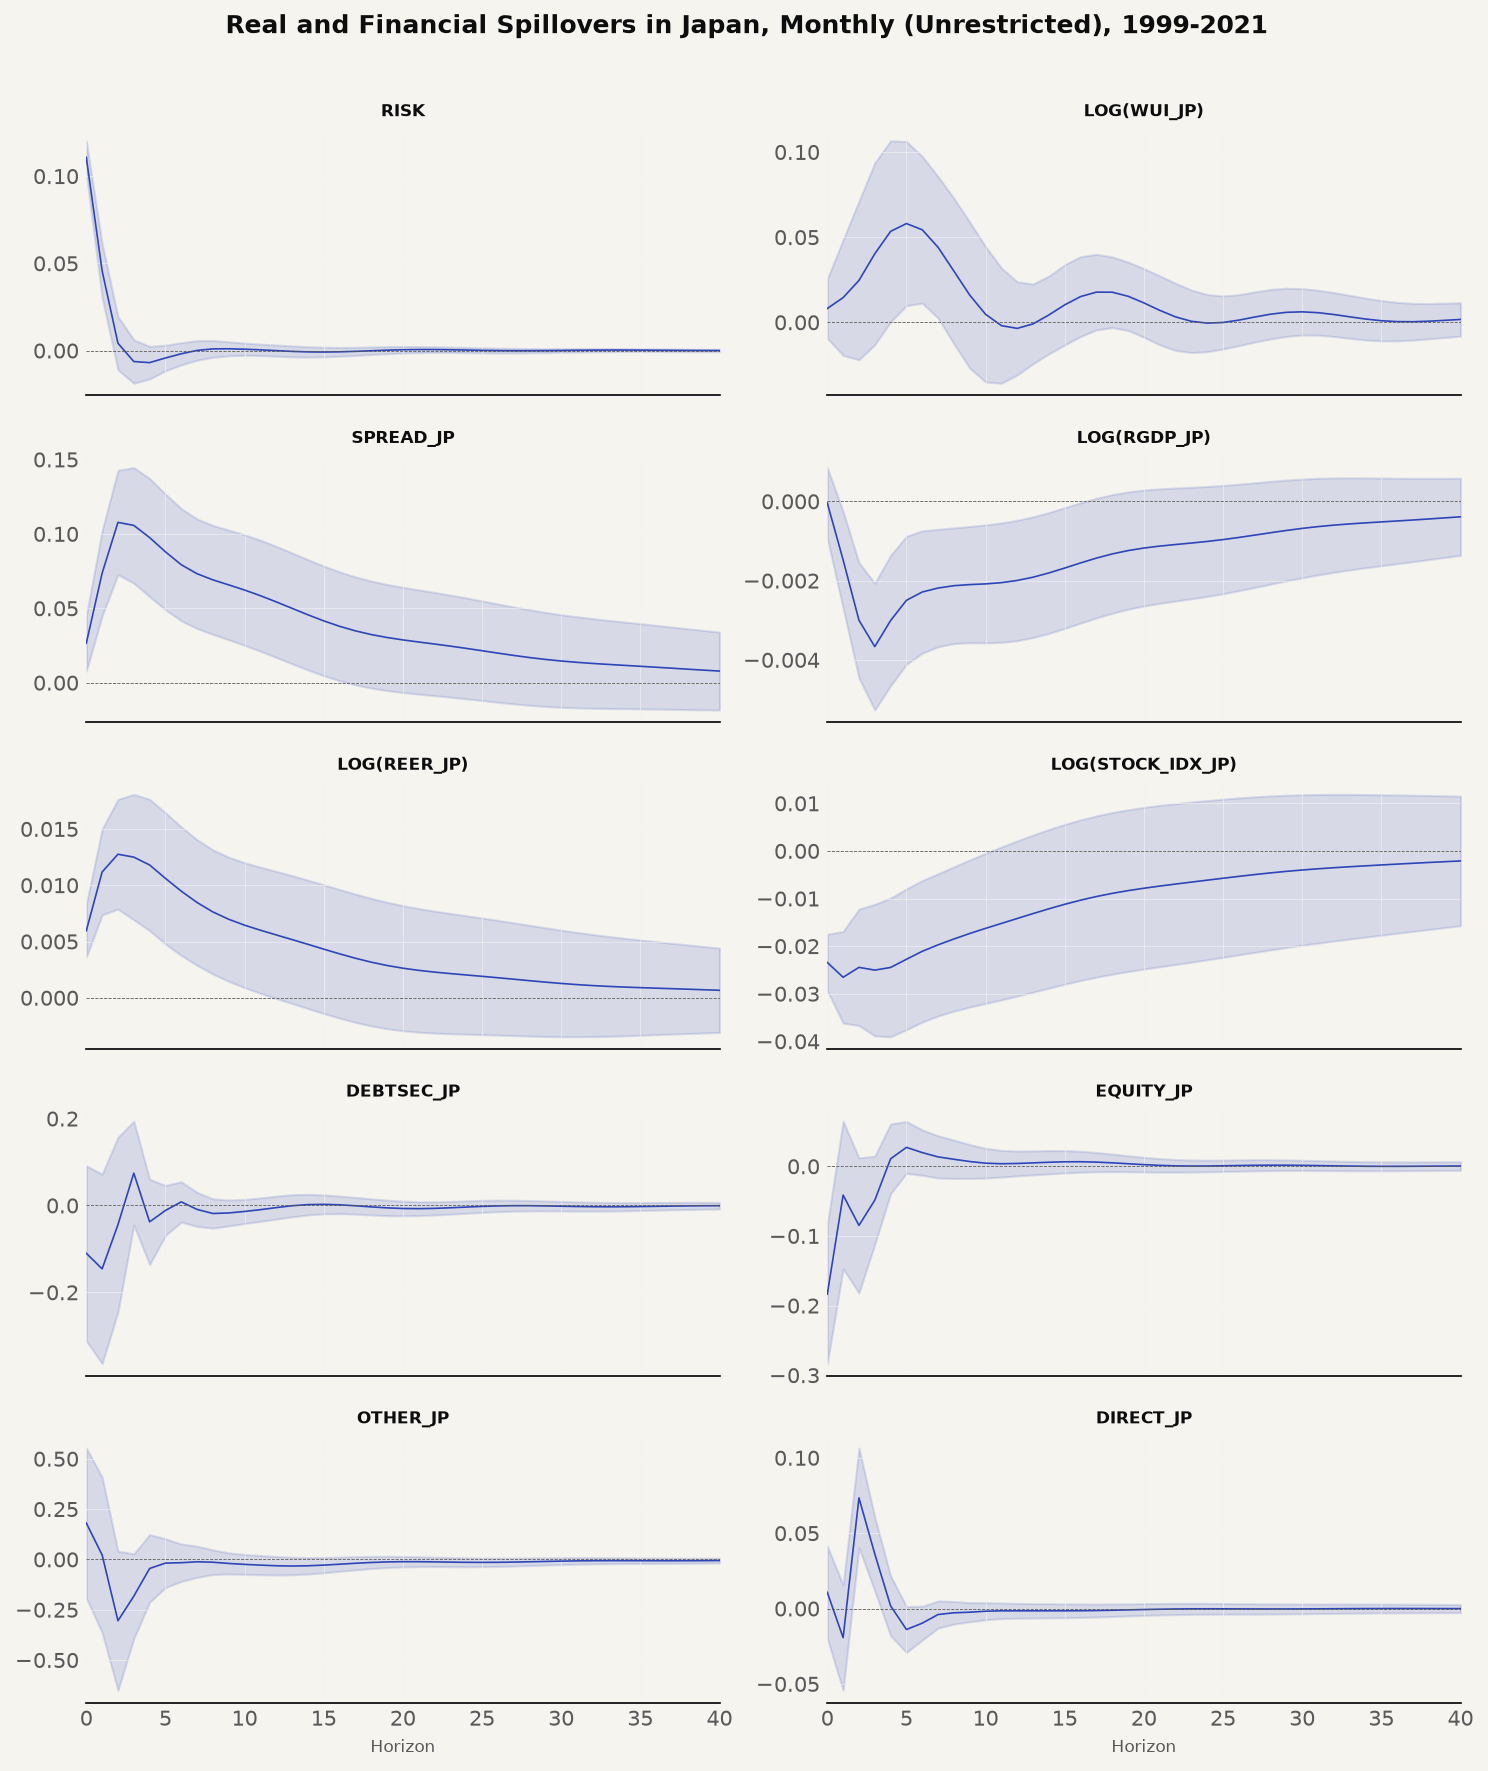
\includegraphics[width=\textwidth]{data/processed/var_results/figures/irf_grid_monthly_unrestricted_paper.png}
  \caption{Monthly Unrestricted Impulse Responses, Paper Period}
  \label{fig:irf_monthly_unrestricted_paper}
\end{figure}

\subsection{Extended Period}

The analysis moves from the paper period to the extended sample. Figures~\ref{fig:irf_daily_extended} and~\ref{fig:irf_monthly_extended} present the daily and monthly restricted grids over the full 1999 to 2026 sample with current-vintage data. The daily RGDP response remains negative and statistically significant, at --0.000630 at day 50 with a band below zero. The monthly extended grid tells the decisive part of the story. The RGDP response at month 3 is --0.000162 with a band spanning zero, against --0.003980 in the paper period, and it remains statistically indistinguishable from zero at every horizon after the impact day. The output channel that the paper identifies for Japan attenuates to statistical indistinguishability at the monthly frequency in the extended sample, while the daily tier retains a significant negative response. The spread channel persists, with the monthly extended spread response at 0.075 at month 3 and significant, and the daily REER response remains positive, at 0.002 at day 50, although the monthly extended REER response at month 3 is 0.004 with a band crossing zero. The price channels survive in weakened form, and the real channel does not.

\begin{figure}[htbp]
  \centering
  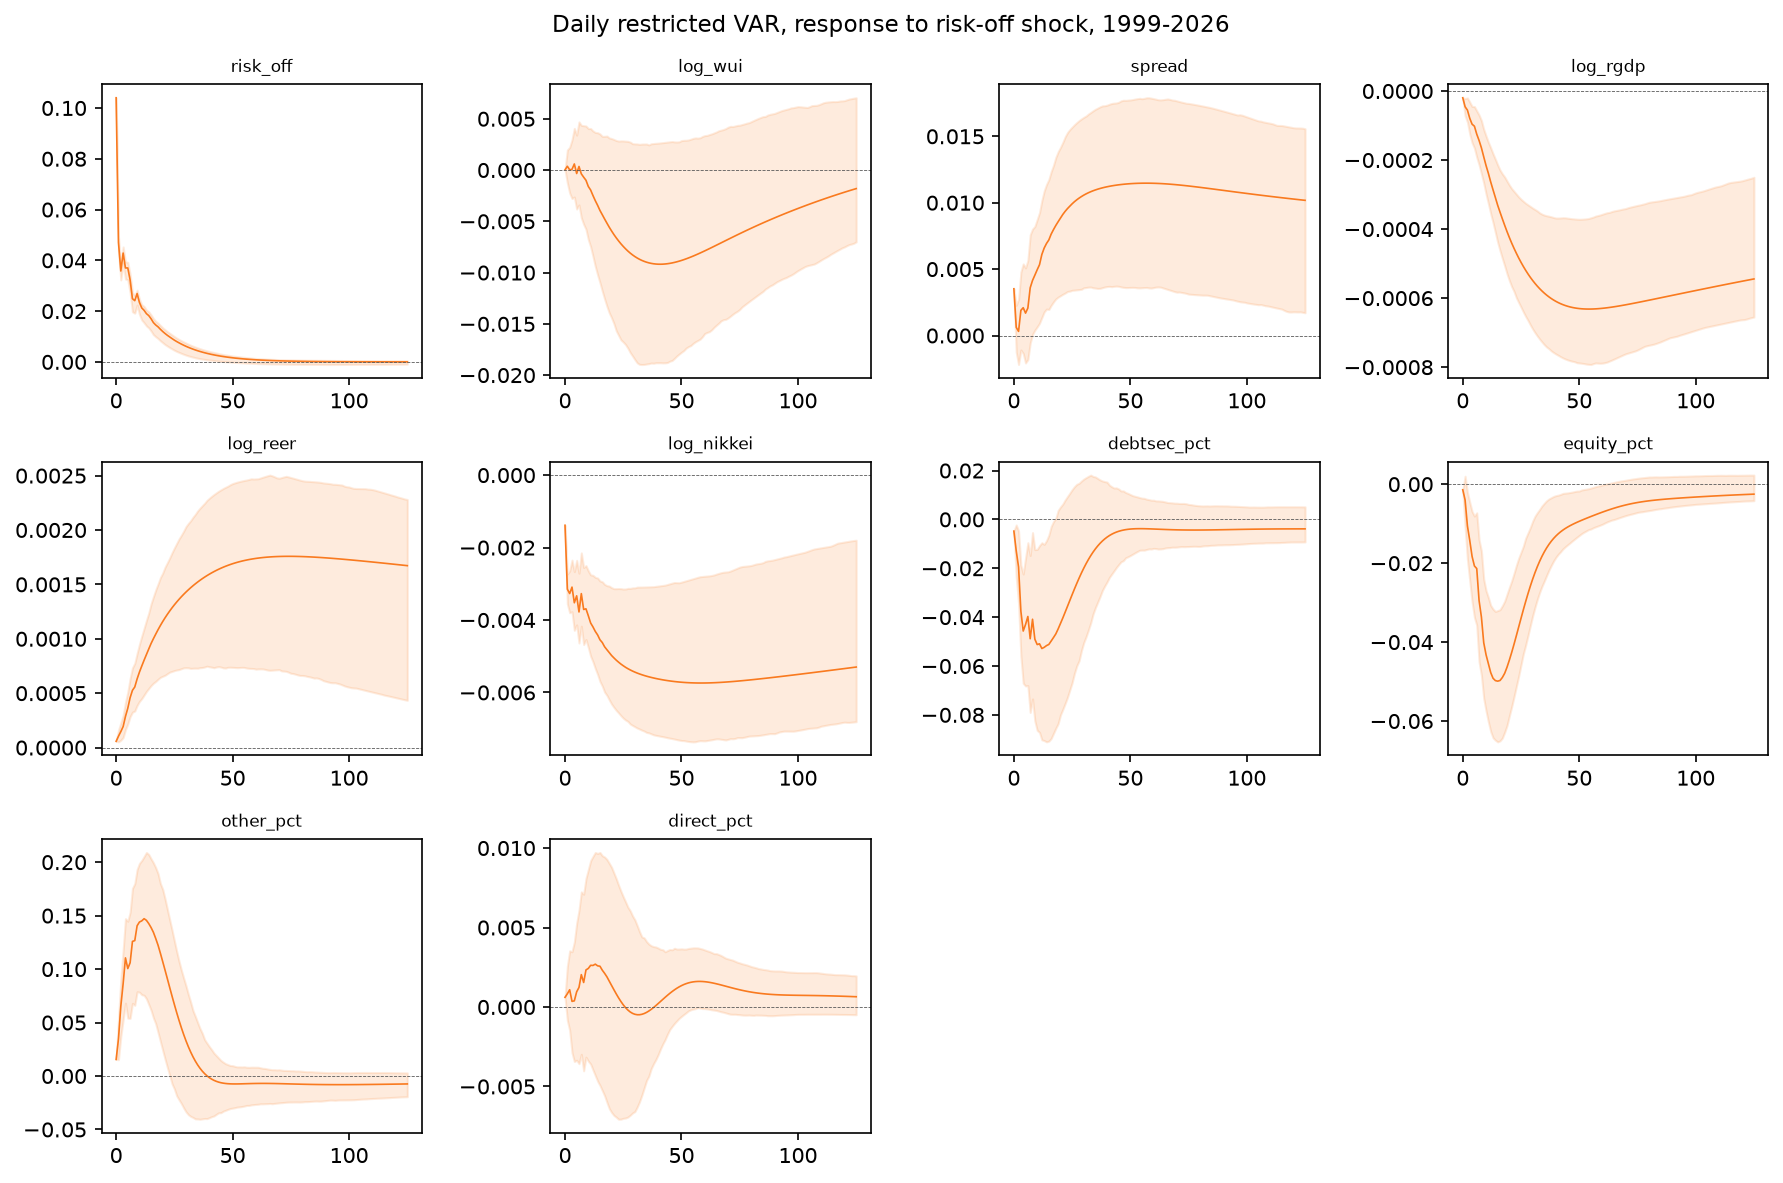
\includegraphics[width=\textwidth]{data/processed/var_results/figures/irf_grid_daily_restricted_extended.png}
  \caption{Daily Restricted Impulse Responses, Extended Sample}
  \label{fig:irf_daily_extended}
\end{figure}

\begin{figure}[htbp]
  \centering
  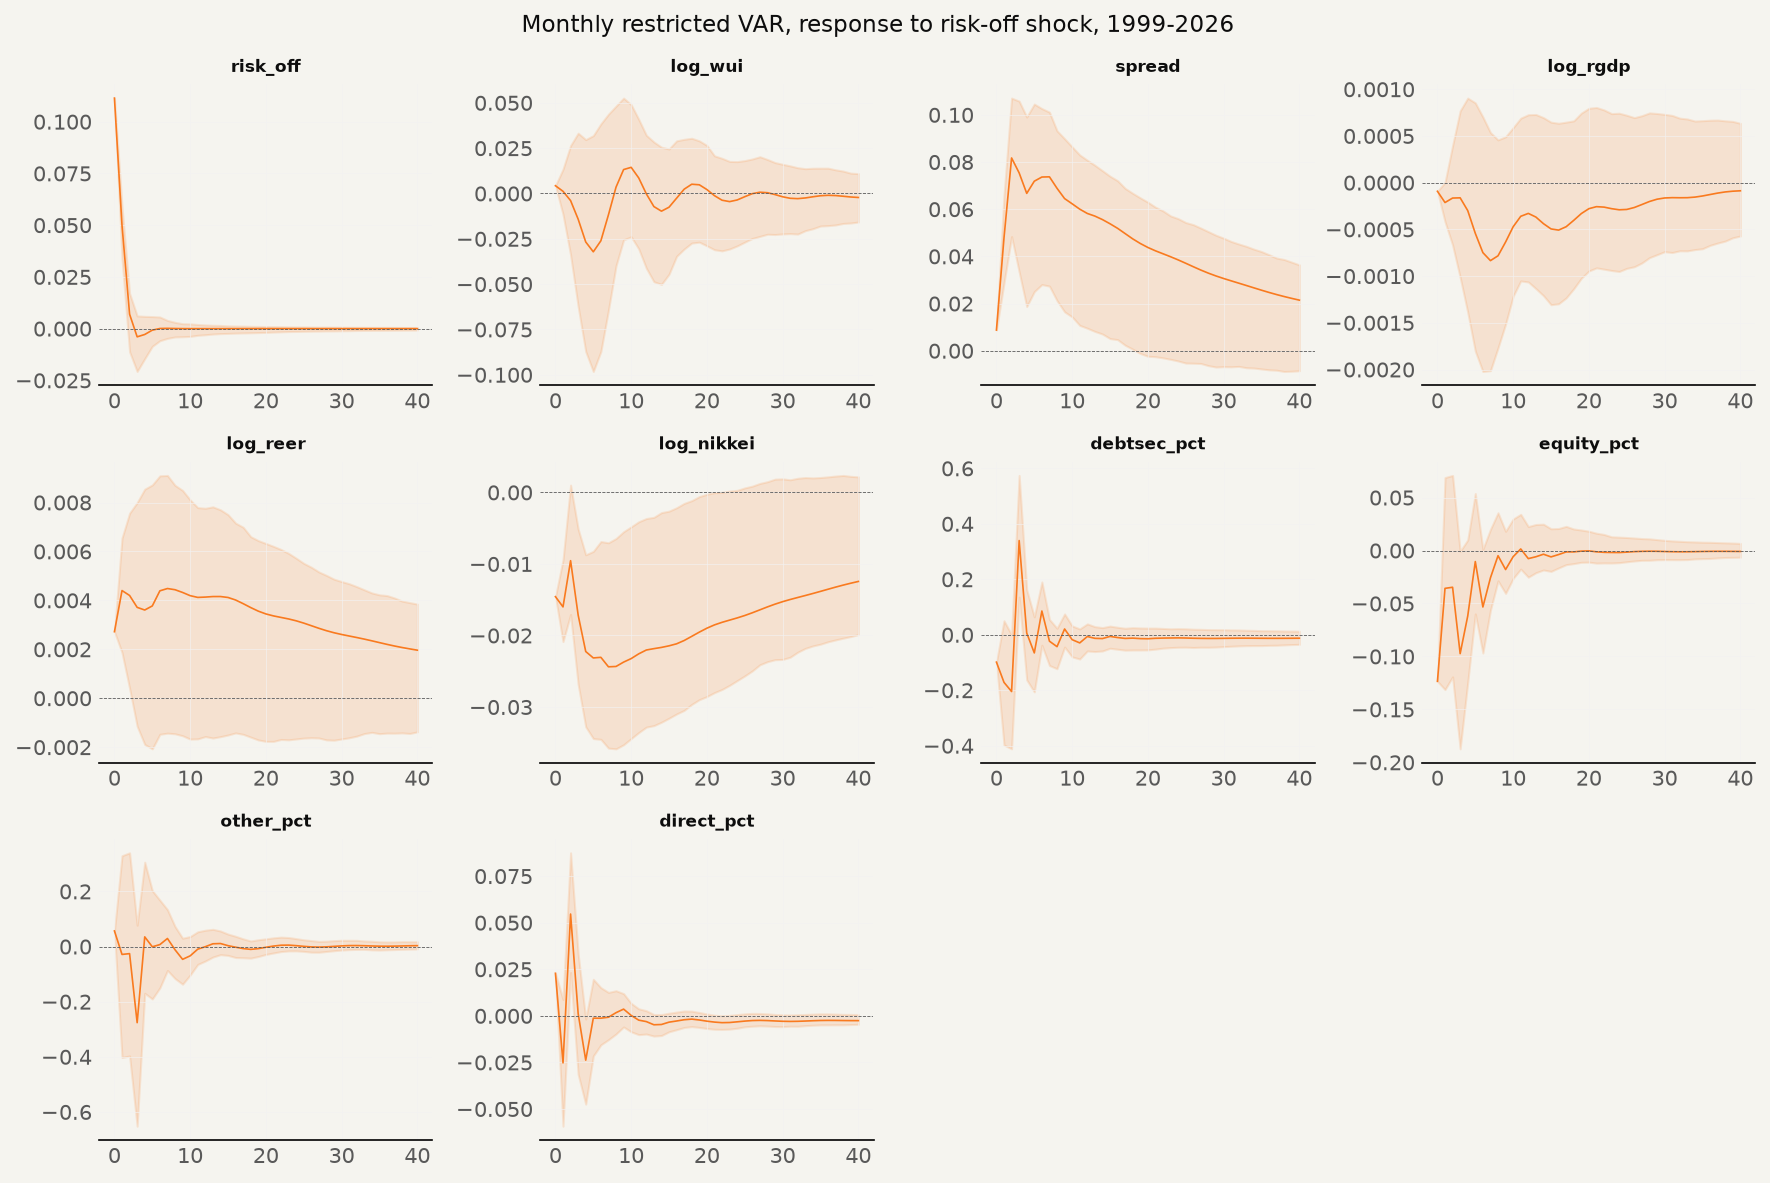
\includegraphics[width=\textwidth]{data/processed/var_results/figures/irf_grid_monthly_restricted_extended.png}
  \caption{Monthly Restricted Impulse Responses, Extended Sample}
  \label{fig:irf_monthly_extended}
\end{figure}

\subsection{Cross-Validation Against the Paper}

The paper-period comparisons reported above are consolidated in Table~\ref{tab:crossval}, which summarizes the comparison of every variable and frequency against the paper's published figures. Of the 17 comparisons, nine are matches, five are partial matches, and three are mismatches. The daily mismatches are the WUI and other investment, and the monthly mismatch is the WUI. A match means the paper's qualitative conclusion reproduces, with sign, shape, and timing in agreement and magnitude differences consistent with software-variant shock scaling. A partial match means the direction or conclusion holds but a meaningful detail diverges, such as an earlier trough, a missing initial blip, or a noisier trajectory. A mismatch means the sign is opposite and no rescaling reconciles the result with the published figure. The paper's weekly panels are not replicated, since the two-tier design covers daily and monthly frequencies only.

\begin{table}[htbp]
  \centering
  \caption{Cross-validation of Impulse Responses, Replication Versus Published Paper}
  \label{tab:crossval}
  \small
  \begin{tabularx}{\textwidth}{@{}l l p{4.6cm} p{4.6cm} l@{}}
    \toprule
    Variable & Frequency & Paper & Replication & Verdict \\
    \midrule
    Risk-off & Daily & 0.10 to 0 by day 25 & 0.098 to 0 by day 125 & MATCH \\
    WUI & Daily & rises to +0.0017 plateau & trough --0.010 at day 40 & MISMATCH \\
    Spread & Daily & peak 0.010 day 50, decays to 0.007 & peak 0.015 day 50, decays to 0.012 & MATCH \\
    RGDP & Daily & trough --0.0006 day 45, recovers to --0.0004 & trough --0.0007 day 50, --0.0006 at day 125 & MATCH \\
    REER & Daily & +0.0008 plateau & +0.002 plateau at day 50 & MATCH \\
    Stock index & Daily & +0.0005 blip, then --0.001, flat --0.0005 & negative from day 0, trough --0.0066 day 50 & PARTIAL \\
    Debtsec & Daily & --0.005 dip, then flat 0 & dip --0.058 day 12, settles near 0 & PARTIAL \\
    Equity & Daily & trough --0.006 day 40, recovers to +0.001 & trough --0.052 day 16, recovers to --0.002 & PARTIAL \\
    Other & Daily & dip, then +0.010 peak day 50 & spike 0.163 day 10, then --0.017 day 50 & MISMATCH \\
    Direct & Daily & --0.002 dip, then +0.001 plateau & +0.0015 day 50, settles near 0.001 & MATCH \\
    WUI & Monthly & +0.002 start, --0.003 dip month 7 & peak 0.052 month 5, oscillates & MISMATCH \\
    RGDP & Monthly & +0.001 start, trough --0.002 months 7--8, recovers to 0 & trough --0.004 month 3, zero by month 24 & PARTIAL \\
    REER & Monthly & +0.004, peak +0.005 months 3--4, ends --0.001 & +0.005 start, peak 0.012 month 3, ends 0.001 & MATCH \\
    Stock index & Monthly & --0.017 start, recovers to --0.004 month 40 & --0.021 start, recovers to 0.0002 month 40 & MATCH \\
    Spread & Monthly & 0.04 start, 0.075 spike month 3, decays to 0.01 & 0.024 start, 0.115 spike month 3, decays to 0.003 & MATCH \\
    Debtsec & Monthly & +0.06 start, volatile, settles to 0 & --0.10 start, volatile, settles to 0 & PARTIAL \\
    Equity & Monthly & trough --0.065 month 4, +0.025 rebound & trough --0.055 month 3, +0.026 rebound & MATCH \\
    \bottomrule
  \end{tabularx}
\end{table}

The full significance record for the capital flow responses is reported in Table~\ref{tab:flowsig}. Of the forty specification-horizon entries, exactly two reach the 95 percent threshold, and both are direct investment at the three-month horizon, under the restricted and unrestricted specifications.

\begin{longtable}{@{}l l r r r r l@{}}
  \caption{Capital Flow Response Significance by Specification and Horizon} \label{tab:flowsig} \\
  \toprule
  Specification & Variable & Horizon & Response & Lower & Upper & Significant \\
  \midrule
  \endfirsthead
  \toprule
  Specification & Variable & Horizon & Response & Lower & Upper & Significant \\
  \midrule
  \endhead
  \bottomrule
  \endlastfoot
  \small
Restricted & Debtsec & 1 & -0.1502 & -0.3680 & 0.0724 & No \\
Restricted & Debtsec & 3 & 0.0755 & -0.0466 & 0.2190 & No \\
Restricted & Debtsec & 6 & 0.0093 & -0.0422 & 0.0695 & No \\
Restricted & Debtsec & 12 & -0.0026 & -0.0264 & 0.0289 & No \\
Restricted & Debtsec & 24 & -0.0021 & -0.0125 & 0.0134 & No \\
Restricted & Equity & 1 & -0.0285 & -0.1217 & 0.0877 & No \\
Restricted & Equity & 3 & -0.0553 & -0.1226 & 0.0268 & No \\
Restricted & Equity & 6 & 0.0175 & -0.0166 & 0.0649 & No \\
Restricted & Equity & 12 & 0.0021 & -0.0128 & 0.0244 & No \\
Restricted & Equity & 24 & -0.0016 & -0.0129 & 0.0082 & No \\
Restricted & Other & 1 & 0.0113 & -0.3867 & 0.3990 & No \\
Restricted & Other & 3 & -0.2186 & -0.4642 & 0.0219 & No \\
Restricted & Other & 6 & -0.0370 & -0.1543 & 0.0806 & No \\
Restricted & Other & 12 & -0.0359 & -0.0877 & 0.0190 & No \\
Restricted & Other & 24 & -0.0149 & -0.0354 & 0.0114 & No \\
Restricted & Direct & 1 & -0.0172 & -0.0492 & 0.0154 & No \\
Restricted & Direct & 3 & 0.0431 & 0.0143 & 0.0673 & Yes \\
Restricted & Direct & 6 & -0.0074 & -0.0206 & 0.0038 & No \\
Restricted & Direct & 12 & -0.0009 & -0.0070 & 0.0044 & No \\
Restricted & Direct & 24 & 0.0003 & -0.0027 & 0.0041 & No \\
Unrestricted & Debtsec & 1 & -0.1460 & -0.3641 & 0.0721 & No \\
Unrestricted & Debtsec & 3 & 0.0744 & -0.0451 & 0.1940 & No \\
Unrestricted & Debtsec & 6 & 0.0082 & -0.0382 & 0.0547 & No \\
Unrestricted & Debtsec & 12 & -0.0049 & -0.0315 & 0.0216 & No \\
Unrestricted & Debtsec & 24 & -0.0037 & -0.0180 & 0.0106 & No \\
Unrestricted & Equity & 1 & -0.0413 & -0.1475 & 0.0648 & No \\
Unrestricted & Equity & 3 & -0.0486 & -0.1119 & 0.0146 & No \\
Unrestricted & Equity & 6 & 0.0197 & -0.0129 & 0.0522 & No \\
Unrestricted & Equity & 12 & 0.0041 & -0.0138 & 0.0219 & No \\
Unrestricted & Equity & 24 & 0.0004 & -0.0079 & 0.0088 & No \\
Unrestricted & Other & 1 & 0.0223 & -0.3641 & 0.4086 & No \\
Unrestricted & Other & 3 & -0.1828 & -0.3936 & 0.0281 & No \\
Unrestricted & Other & 6 & -0.0164 & -0.1097 & 0.0770 & No \\
Unrestricted & Other & 12 & -0.0315 & -0.0775 & 0.0144 & No \\
Unrestricted & Other & 24 & -0.0144 & -0.0366 & 0.0078 & No \\
Unrestricted & Direct & 1 & -0.0193 & -0.0543 & 0.0156 & No \\
Unrestricted & Direct & 3 & 0.0362 & 0.0117 & 0.0607 & Yes \\
Unrestricted & Direct & 6 & -0.0097 & -0.0210 & 0.0015 & No \\
Unrestricted & Direct & 12 & -0.0015 & -0.0064 & 0.0034 & No \\
Unrestricted & Direct & 24 & -0.0002 & -0.0038 & 0.0034 & No \\
  \bottomrule
\end{longtable}

\begin{center}
  \small\textit{Note.} Monthly restricted and unrestricted specifications, paper period. Responses are percentage points of nominal GDP. A response is significant when the 95 percent Monte Carlo band excludes zero.
\end{center}


How close the replication got is summarized by the numbers themselves. The risk-off impulse matches to three decimal places. The RGDP trough is 1.2 times deeper and arrives five days later, well inside the uncertainty envelope of unreported software settings. The spread peak is 1.5 times larger with the same timing and persistence. The REER plateau is 2.5 times larger with the same direction. The monthly RGDP trough is twice as deep and four to five months earlier, and the equity trough matches to within a hundredth of a percentage point. The two daily mismatches and the monthly WUI mismatch are the honest boundary of the replication, and each has a documented mechanism, the frequency fragility of the uncertainty index and the source-data sensitivity of the other investment category. Section 5 interprets these results against the theoretical framework of Section 2 and assesses the five hypotheses.
